\documentclass[custom,grid]{flashcards}
\usepackage[T1]{fontenc} % better support for characters with accents and non-English characters
\usepackage[utf8]{inputenc} % tegnsæt
\usepackage[danish]{babel}
%\usepackage[latin1]{inputenc}
\usepackage[pdftex]{graphicx} % figurer
\usepackage{amsfonts}
\usepackage{amsmath}
\usepackage{MinionPro}
\usepackage{tikz}
\usetikzlibrary{calc,patterns,decorations.pathmorphing,decorations.markings,matrix,arrows}
\usepackage{mathtools} % udvidet matematisk typesetting pakke
\usepackage{bm} % til bold text
\usepackage{mhchem}
\usepackage{chemmacros}
\usepackage{chemfig}
\usepackage{color}
\usepackage{modiagram}
\usepackage{tabularx}

\usepackage{epstopdf}
\epstopdfDeclareGraphicsRule{.tiff}{png}{.png}{convert #1 \OutputFile}
\AppendGraphicsExtensions{.tiff}

\cardfrontstyle[\large]{headings}
\cardbackstyle{plain}
\setlength{\cardmargin}{0.8cm}

\begin{document}
% Fremstilling
% Struktur
% Reaktion
% Egenskab
% Anvendelse
% Trend
% Teori
%\cardfrontfoot{Kapitel 9}
\begin{flashcard}[Trend]{Hvilken type bindinger danner grundstofferne i 5. hovedgruppe?}
Nitrogen og fosfor laver covalente bindinger. Arsen laver netværk-covalente bindinger. Antimon og bismuth laver metalliske bindinger.
\end{flashcard}

\begin{flashcard}[Trend]{Hvilken type bindinger danner grundstofferne i 2. periode?}
\begin{tabular}{ c | c | c | c | c | c | c | c }
\ce{Li} & \ce{Be} & \ce{B} & \ce{C} & \ce{N2} & \ce{O2} & \ce{F2} & \ce{Ne} \\ \hline
M & M & NC & NC & C & C & C & C
\end{tabular}\\ \vspace{7pt}
M = metallisk, NC = netværk covalent, C = covalent
\end{flashcard}

\begin{flashcard}[Trend]{Hvilken type bindinger danner grundstofferne i 3. periode?}
\begin{tabular}{ c | c | c | c | c | c | c | c }
\ce{Na} & \ce{Mg} & \ce{Al} & \ce{Si} & \ce{P4} & \ce{S8} & \ce{Cl2} & \ce{Ar} \\ \hline
M & M & M & NC & C & C & C & C
\end{tabular}\\ \vspace{7pt}
M = metallisk, NC = netværk covalent, C = covalent
\end{flashcard}

\begin{flashcard}[Trend]{Hvilken bindingstype er der tale om i de højeste flourider af grundstofferne i 2. periode?}
\begin{tabular}{ c | c | c | c | c | c }
\ce{LiF} & \ce{BeF2} & \ce{BF3} & \ce{CF4} & \ce{NF3} & \ce{OF2} \\ \hline
I & NC & C & C & C & C
\end{tabular}\\ \vspace{7pt}
I = ionisk, NC = netværk covalent, C = covalent
\end{flashcard}

\begin{flashcard}[Trend]{Hvilken bindingstype er der tale om i de højeste flourider af grundstofferne i 3. periode?}
\begin{tabular}{ c | c | c | c | c | c | c }
\ce{NaF} & \ce{MgF2} & \ce{AlF3} & \ce{SiF4} & \ce{PF5} & \ce{SF6} & \ce{ClF5} \\ \hline
I & I & NC & C & C & C & C
\end{tabular}\\ \vspace{7pt}
I = ionisk, NC = netværk covalent, C = covalent
\end{flashcard}

\begin{flashcard}[Trend]{Hvilken bindingstype er der tale om i de højeste oxider af grundstofferne i 2. periode?}
\begin{tabular}{ c | c | c | c | c | c }
\ce{Li2O} & \ce{BeO} & \ce{B2O3} & \ce{CO2} & \ce{N2O5} & \ce{F2O} \\ \hline
I & I & NC & C & C & C
\end{tabular}\\ \vspace{7pt}
I = ionisk, NC = netværk covalent, C = covalent
\end{flashcard}

\begin{flashcard}[Trend]{Hvilken bindingstype er der tale om i de højeste oxider af grundstofferne i 3. periode?}
\begin{tabular}{ c | c | c | c | c | c | c }
\ce{Na2O} & \ce{MgO} & \ce{Al2O3} & \ce{SiO2} & \ce{P4O10} & \ce{(SO3)3} & \ce{Cl2O7} \\ \hline
I & I & I & NC & C & C & C
\end{tabular}\\ \vspace{7pt}
I = ionisk, NC = netværk covalent, C = covalent
\end{flashcard}

\begin{flashcard}[Trend]{Hvilken bindingstype er der tale om i hydriderne af grundstofferne i 2. periode?}
\begin{tabular}{ c | c | c | c | c | c | c }
\ce{LiH} & \ce{(BeH2)_{$x$}} & \ce{B2H6} & \ce{CH4} & \ce{NH3} & \ce{H2O} & HF \\ \hline
I & NC & C & C & C & C & C
\end{tabular}\\ \vspace{7pt}
I = ionisk, NC = netværk covalent, C = covalent
\end{flashcard}

\begin{flashcard}[Trend]{Hvilken bindingstype er der tale om i hydriderne af grundstofferne i 3. periode?}
\begin{tabular}{ c | c | c | c | c | c | c }
\ce{NaH} & \ce{MgH2} & \ce{(AlH3)_{$x$}} & \ce{SiH4} & \ce{PH3} & \ce{H2S} & \ce{HCl} \\ \hline
I & I & NC & C & C & C & C
\end{tabular}\\ \vspace{7pt}
I = ionisk, NC = netværk covalent, C = covalent
\end{flashcard}

\begin{flashcard}[Trend]{Angiv syre/base egenskaberne af de højeste oxider af grundstofferne i 3. periode}
\begin{tabular}{ c | c | c | c | c | c | c }
\ce{Na2O} & \ce{MgO} & \ce{Al2O3} & \ce{SiO2} & \ce{P4O10} & \ce{(SO3)3} & \ce{Cl2O7} \\ \hline
B & B & A & S & S & S & S
\end{tabular}\\ \vspace{7pt}
B = basisk, S = sur, A = amfoter
\end{flashcard}

\begin{flashcard}[Trend]{Angiv syre/base egenskaberne af de højeste oxider af grundstofferne i 5. hovedgruppe}
\begin{tabular}{ c | c | c | c | c }
\ce{N2O5} & \ce{P4O10} & \ce{As2O3} & \ce{Sb2O3} & \ce{Bi2O3} \\ \hline
S & S & A & A & B
\end{tabular}\\ \vspace{7pt}
B = basisk, S = sur, A = amfoter
\end{flashcard}
%\cardfrontfoot{Kapitel 10}
\begin{flashcard}[Fremstilling]{Hvorledes kan \ce{H2} fremstilles industrielt og i laboratoriet?}
Industrielt:\\ \ce{CH4 + H2O -> CO + 3 H2} \\ \ce{CO + H2O ->[\text{$\Delta$}] CO2 + H2} \\ \ce{K2CO3 + CO2 + H2O -> 2KHCO3} \\ \vspace{7pt}
I laboratoriet: \\ \ce{Zn(s) + 2HCl -> ZnCl2 + H2} \\ \vspace{7pt} samt ved elektrolyse i begge tilfælde:\\
\ce{2 H2O + 2e- -> 2 OH- + H2}\\
\ce{6H2O -> 4H3O+ + O2 + 4e-}
\end{flashcard}

\begin{flashcard}[Trend]{Stiger eller falder reaktiviteten mellem \ce{H2} og halogenerne ned gennem 7. hovedgruppe?}
Reaktiviteten mellem dihydrogen og halogenerne falder ned gennem 7. hovedgruppe.
\end{flashcard}

\begin{flashcard}[Reaktion]{Beskriv hvordan \ce{H2} kan anvendes som reduktionsmiddel}
\ce{H2} kan anvendes på organiske forbindelser:\\
\begin{align*}
\ce{H2\OX{rf1,\ox{-2,\ce{C}}}=\OX{rf2,\ox{-2,\ce{C}}}H2 + \OX{of1,\ox{0,\ce{H2}}} -> \OX{oe1,\ox{+1,\ce{H3}}}\OX{re1,\ox{-3,\ce{C}}}-\OX{re2,\ox{-3,\ce{C}}}\OX{oe2,\ce{H3}}}
\redox(of1,oe2){\small oxidation}
\redox(of1,oe1){}
\redox(rf1,re2)[][-1]{\small reduktion}
\redox(rf2,re1)[][-1]{}
\end{align*} \\ \vspace{7pt}
samt uorganiske, herunder metaloxider:\\
\begin{align*}
\ce{\OX{rf1,\ox{+2,\ce{Cu}}} O + \OX{of1,\ox{0,\ce{H2}}} -> \OX{re1,\ox{0,\ce{Cu}}} + \OX{oe1,\ox{+1,\ce{H2}}} O}
\redox(of1,oe1){\small oxidation}
\redox(rf1,re1)[][-1]{\small reduktion}
\end{align*}
\end{flashcard}

\begin{flashcard}[Trend]{Hvorledes kan hydriderne af grundstofferne i det periodiske system karakteriseres som henholdsvis ioniske, kovalente eller metalliske?}
Hydriderne af grundstofferne i 1. og 2. hovedgruppe kan karakteriseres som ioniske. \\
Hydriderne af overgangsmetallerne kan karakteriseres som metalliske. \\
Hydriderne af grundstofferne i 3. til 7. hovedgruppe kan karakteriseres som covalente.
\end{flashcard}

\begin{flashcard}[Egenskab]{Begrund hvorfor vands og flussyres kogepunkt er væsentligt højere end forventet}
Intermolekylære hydrogenbindinger.
\end{flashcard}

\begin{flashcard}[Reaktion]{Færdiggør og afstem\\ \vspace{7pt}
\ce{H2 + Na -> NaH}\\
\ce{H2 + F2 -> HF}\\
\ce{H2 + O2 -> H2O}\\
\ce{H2 + N2 -> NH3}\\
\ce{H2 + CuO ->[\text{$\Delta$}] Cu}}

\ce{H2 + 2Na -> 2NaH}\\
\ce{H2 + F2 -> 2HF}\\
\ce{2H2 + O2 -> 2H2O}\\
\ce{3H2 + N2 -> 2NH3}\\
\ce{H2 + CuO ->[\text{$\Delta$}] Cu + H2O}
\end{flashcard}
%\cardfrontfoot{Kapitel 11}
\begin{flashcard}[Reaktion]{Beskriv henholdsvis lithiums reaktion med atmosfæren (oxygen og kuldioxid) samt alkalimetallernes reaktion med vand}

\ce{4Li + O2 -> 2Li2O}\\
\ce{Li2O + CO2 -> Li2CO3}\\ \vspace{7pt}
\ce{2K + 2H2O -> 2KOH + H2}\\
ligeledes for de andre.
\end{flashcard}

\begin{flashcard}[Egenskab]{Forklar hvorfor \ce{Li+} er exceptionel god til at koordinere vand}
\ce{Li+} har godt nok kun én positiv ladning. Til gengæld er Van der Walls radius af ionen relativt lille hvilket fører til en relativt høj ladningstæthed (ladning pr. volumen). Det er ladningstætheden der afgører ionens evne til at koordinere vand.
\end{flashcard}

\begin{flashcard}[Egenskab]{Opskriv alkalimetallernes flammefarver}
\begin{tabular}{ l l }
Lithium & \color{red}Rød \\
Natrium & \color{yellow}Gul \\
Kalium & \color{violet}Lilla \\
Rubidium & \color{red}Rød-violet \\
Cesium & \color{blue}Blå
\end{tabular}
\end{flashcard}

\begin{flashcard}[Egenskab]{Hvilken sammenhæng er der mellem opløseligheden af et salt, kationens radius og anionens radius?}
Kationer og anioner af nogenlunde samme størrelse vil have lettere ved at skabe et stabilt gitter (krystal, bundfald) end kationer og anioner med vidt forskellige størrelser. Derfor vil salte af ioner med stor størrelsesmæssig forskel ofte være let opløselige. Eksempelvis \ce{LiI}.
\end{flashcard}

\begin{flashcard}[Reaktion]{Opskriv reaktionen mellem nitrogen og et alkalimetal der har en rød flammefarve og høj ladningstæthed. Opskriv da produktets reaktion med vand.}
\ce{6Li + N2 -> 2Li3N} \\ \vspace{7pt}
\ce{Li3N + 3H2O -> NH3 + 3LiOH}
\end{flashcard}

\begin{flashcard}[Anvendelse]{Beskriv med ord og reaktionsskema hvorledes lithium indgår i genopladelige Lithium-Ion batterier}
Anoden består af \ce{LiCoO2(s)} og katoden af grafit. Ved opladning bevæger \ce{Li+} ioner sig fra anoden til katoden hvor de interkaleres i grafit katoden.\\ \vspace{7pt}
\ce{LiCoO2 -> Li_{($1-x$)}CoO2 + $x$Li+ + $x$e-} \\
\ce{C + $x$Li+ + $x$e- -> Li_{$x$}C} \\ \vspace{7pt}
Den modsatte reaktion finder sted ved afladning.
\end{flashcard}

\begin{flashcard}[Anvendelse]{Beskriv med reaktionsskema hvorledes lithium indgår i ikke-genopladelige batterier}
De har alle lithiums ionisering (anodereaktionen) til fælles: \ce{Li -> Li+ + e-}\\ \vspace{7pt}
Katodereaktionerne varierer batterityperne imellem. Her er tre forskellige batteritypers katodereaktion: \\
\ce{2SOCl2 + 4e- -> 4Cl- + SO2 + S} \\
\ce{SO2Cl2 + 2e- -> 2Cl- + SO2} \\
\ce{2SO2 + 2e- -> S2O4^{-2}}
\end{flashcard}

\begin{flashcard}[Fremstilling]{Opskriv hvordan titanium fremstilles industrielt}
\ce{TiCl4 + 4Na -> 4NaCl + Ti}
\end{flashcard}

\begin{flashcard}[Fremstilling]{Opskriv hvordan natrium og kalium fremstilles industrielt}
Natrium fremstilles ved elektrolyse af natriumchloridopløsning \\ \vspace{7pt}
\ce{Na+ + e- -> Na} \\
\ce{2Cl- -> Cl2 + 2e-} \\ \vspace{7pt}
Kalium fremstilles ved følgende reaktion ved $850\,^{\circ}{\rm C}$ \\
\ce{Na(l) + KCl(l) -> K(g) + NaCl(l)}
\end{flashcard}

\begin{flashcard}[Fremstilling]{Opskriv hvordan natriumhydroxid fremstilles industrielt}
Elektrolyse af natriumchloridopløsning \\ \vspace{7pt}
\ce{2H2O + 2e- -> H2 + 2OH-} \\
\ce{2Cl- -> Cl2 + 2e-} \\ \vspace{7pt}
De dannede hydroxid ioner er forhindret i at kommer i kontakt med chlorgassen af et diaphragm hvor natriumchloridopløsningen kan passere.
\end{flashcard}

\begin{flashcard}[Reaktion]{Opskriv oxiderne af alkalimetallerne samt deres reaktion med vand}
\ce{Li2OH}, \ce{Na2O2}, \ce{KO2}. \\ \vspace{7pt}
\ce{Li2O + H2O -> 2LiOH} \\
\ce{Na2O2 + 2H2O -> 2NaOH + H2O2} \\
\ce{2KO2 + 2H2O -> 2KOH + H2O2 + O2}
\end{flashcard}

\begin{flashcard}[Anvendelse]{Beskriv med reaktionsligninger hvorledes \ce{KO2} kan bruges til at oplagre kuldioxid}
\ce{4KO2 + 2CO2 -> 2K2CO3 + 3O2} \\
\ce{K2CO3 + H2O + CO2 -> 2KHCO3}
\end{flashcard}

\begin{flashcard}[Generelt]{Er dioxid(2-)ionen para- eller diamagnetisk? Begrund med MO teori.}
$2p$ elektronerne danner følgende molekylorbitaler
\begin{MOdiagram}[style=fancy,labels,AO-width=8pt,labels-fs=\footnotesize]
\atom[\ce{O-}]{left}{2p={;pair,pair,up}}
\atom[\ce{O-}]{right}{2p={;pair,pair,up}}
\molecule[\ce{O2^{-2}}]{2pMO={1.3,.4;pair,pair,pair,pair,pair,}}
\end{MOdiagram}\\[-5pt]Diamagnetisk, ingen uparrede elektroner.
\end{flashcard}

\begin{flashcard}[Generelt]{Er dioxid(1-)ionen para- eller diamagnetisk? Begrund med MO teori.}
$2p$ elektronerne danner følgende molekylorbitaler
\begin{MOdiagram}[style=fancy,labels,AO-width=8pt,labels-fs=\footnotesize]
\atom[\ce{O-}]{left}{2p={;pair,pair,up}}
\atom[\ce{O-}]{right}{2p={;pair,up,up}}
\molecule[\ce{O2^{-2}}]{2pMO={1.3,.4;pair,pair,pair,pair,up,}}
\end{MOdiagram}\\[-5pt]Paramagnetisk, uparrede elektroner i $2\pi^{*}$.
\end{flashcard}

\begin{flashcard}[Reaktion]{Opskriv reaktionen mellem aluminium metal og hydroxidionen}
\ce{2Al + 2OH- + 6H2O -> 2[Al(OH)4]- + 3H2}
\end{flashcard}

\begin{flashcard}[Reaktion]{Hvad sker der med en natriumhydroxidopløsning uden låg?}
\ce{OH- + CO2 -> HCO3- }
\end{flashcard}

\begin{flashcard}[Reaktion]{Salte af alkalimetalionerne samt ammoniumionen er normalt letopløselige. Som de eneste er alkalimetalionerne f.eks. letopløselige som carbonater. Opskriv reaktioner hvorved \ce{Na+}, \ce{K+} og \ce{NH4+} kan bundfældes}
Natrium\\
\ce{Na+ + [Sb(OH)6]- -> Na[Sb(OH)6](s)} \\ \vspace{7pt}
Kalium og ammonium\\
\ce{3K+ + [Co(NO)6]^{3-} -> K3[Co(NO)6](s)}\\
\ce{3NH4+ + [Co(NO)6]^{3-} -> (NH4)3[Co(NO)6](s)}
\end{flashcard}

\begin{flashcard}[Anvendelse]{Beskriv med reaktionsskemaer hvorledes natriumbicarbonat anvendes i bagepulver}
Bagepulver består af \ce{NaHCO3} samt \ce{Ca(H2PO4)2}.\\ \vspace{7pt}
\ce{2NaHCO3 + Ca(H2PO4)2 ->[\text{$\Delta$}] NaHPO4 + CaHPO4 + 2CO2 + 2H2O}
\end{flashcard}

\begin{flashcard}[Reaktion]{Hvad sker der med natriumbicarbonat når det opvarmes?}
\ce{2NaHCO3 -> Na2CO3 + CO2 + H2O}
\end{flashcard}

\begin{flashcard}[Egenskab]{Beskriv med ord og reaktionsskema hvad der sker når et alkalimetal, i dette tilfælde natrium,  opløses i ammoniak}
\ce{Na(s) -> Na+(ammoniak) + e^{-}(ammoniak)}\\
Opløsningen vil have en dyb blå farve når den er tynd og en bronze farve når det er koncentreret. Med tiden vil natrium reagere med ammoniak og danne natriumamid\\
\ce{2Na+ + 2NH3 + 2e- -> 2NaNH2 + H2}
\end{flashcard}

\begin{flashcard}[Fremstilling]{Hvordan findes kaliumchlorid i naturen og hvordan udvindes det?}
\ce{KCl} findes bl.a. som \ce{KMgCl3\cdot 6H2O} samt \ce{MgSO4\cdot H2O}. Udvindes v. 3 forskellige metoder.\\
\begin{itemize}
\item Udnyt forskellige opløsligheder af saltene ved at opløse dem. Energikrævende at fordampe vand.
\item Opløs i saltlage. Blæs luft igennem. \ce{KCl} sidder fast på boblernes overflade som opfanges.
\item Elektrostatisk proces. Mal krystaller til pulver og giv dem ladning via. friktion. De kan herefter adskilles.
\end{itemize}
\end{flashcard}

\begin{flashcard}[Fremstilling]{Fra hvilket mineral og hvordan udvindes \ce{Na2CO3}?}
Trona: \ce{Na2CO3\cdot NaHCO3 \cdot 2H2O}\\ \vspace{7pt}
Opvarmning, rekrystallisation, opvarmning\\
\ce{2Na2CO3\cdot NaHCO3 \cdot 2H2O ->[\text{$\Delta$}] 3Na2CO3 + 5H2O + CO2}\\
Natriumcarbonat genopløses hvorved faste urenheder filtreres fra. \ce{Na2CO3\cdot H2O} opnås ved tørring.\\
\ce{Na2CO3\cdot H2O ->[\text{$\Delta$}] Na2CO3 + H2O(g)}
\end{flashcard}

\begin{flashcard}[Fremstilling]{Beskriv hvorledes \ce{Na2CO3} kan fremstilles ud fra Solvay processen}
\ce{2NaCl + CaCO3 <=> Na2CO3 + CaCl2}
\end{flashcard}

\begin{flashcard}[Anvendelse]{Beskriv med reaktionsskema hvorledes \ce{Na2CO3} anvendes i produktionen af glas.}
\ce{Na2CO3 + $x$SiO2 ->[\text{$\Delta$}] Na2O\cdot $x$SiO2 + CO2 }
\end{flashcard}
%\cardfrontfoot{Kapitel 12}
\begin{flashcard}[Teori]{Begrund at magnesium(II) har en mindre ionradius end natrium(I)}
Begge ioner har den samme elektronkonfiguration $1s^{2}2s^{2}2p^{6}$\\ \vspace{7pt}
Dog har magnesium én proton mere end natrium. Det betyder, at magnesium kan udøve en større tiltrækkende kraft på elektronerne således at de befinder sig tættere på kernen.
\end{flashcard}

\begin{flashcard}[Reaktion]{Opskriv reaktionen mellem en (for det meste) intert gas og magnesium metal}
\ce{3Mg + N2 -> Mg3N2}
\end{flashcard}

\begin{flashcard}[Egenskab]{Angiv hvilke af jordalkalimetallerne der er opløselige med \ce{CO3^{2-}}, \ce{PO4^{3-}}, \ce{SO4^{2-}} og \ce{OH-}}
\begin{tabular}{ r|c|c|c|c| }
 \multicolumn{1}{r}{}
  & \multicolumn{1}{c}{\ce{CO3^{2-}}}
  & \multicolumn{1}{c}{\ce{PO4^{3-}}}
  & \multicolumn{1}{c}{\ce{SO4^{2-}}}
  & \multicolumn{1}{c}{\ce{OH-}}
  
   \\
 \cline{2-5}
 \ce{Mg^{2+}}& & & Opløselig & \\
 \cline{2-5}
 \ce{Ca^{2+}} & & & (Opløselig) & (Opløselig) \\
 \cline{2-5}
 \ce{Sr^{2+}} & & & & Opløselig \\
 \cline{2-5}
 \ce{Ba^{2+}} & & & & Opløselig \\
 \cline{2-5}
 \end{tabular}
\end{flashcard}

\begin{flashcard}[Reaktion]{Vis med reaktionsskema at berylliumoxid er amfotert}
\ce{BeO + 2H3O+ + H2O -> [Be(OH2)4]^{2+}}\\ \vspace{7pt}
\ce{BeO + 2OH- + H2O -> [Be(OH)4]^{2-}}
\end{flashcard}

\begin{flashcard}[Teori]{Begrund hvorfor beryllium har tendens til at danne covalente forbindelser}
Beryllium er relativt elektronegativ. Man kan forudsige bindingskarakter ud fra elektronegativitet. Et eksempel er \ce{BeCl2}. Forskellen mellem elektronegativitet for disse er $3.16-1.57=1.59$ hvilket svarer til en polær kovalent binding.
\end{flashcard}

\begin{flashcard}[Struktur]{Optegn strukturen af \ce{[Be(OH2)4]^{2+}}}
\schemestart
$\chemleft[\chemfig{Be(-[2]\ce{OH2})(-[5]\ce{H2O})(<[:-50]\ce{OH2})(<:[:-12]\ce{OH2})}\chemright]^{2+}$
\schemestop
\end{flashcard}

\begin{flashcard}[Fremstilling]{Hvordan findes magnesium i naturen?}
Magnesium findes i naturen som \ce{KMgCl3\cdot 6H2O}, \ce{CaMg(CO3)2} og \ce{MgSO4\cdot 7H2O}
\end{flashcard}

\begin{flashcard}[Reaktion]{Opskriv reaktion for forbrænding af magnesium metal med oxygen henholdsvis carbondioxid}
\ce{2Mg + O2 -> 2MgO} \\ \vspace{7pt}
\ce{2Mg + CO2 -> 2MgO + C}
\end{flashcard}

\begin{flashcard}[Fremstilling]{Beskriv den industrielle fremstilling af magnesium}
\ce{Ca(OH)2 + Mg^{2+} -> Mg(OH2)(s) + Ca^{2+}} \\
\ce{Mg(OH)2 + 2HCl -> MgCl2(aq) + 2H2O} \\
Elektrolyse af \ce{MgCl2} giver \ce{Mg} ved katoden og chlorgas ved anoden. Chlorgas kan genbruges til at danne saltsyre.
\end{flashcard}

\begin{flashcard}[Reaktion]{Hvad sker der når \ce{CaCO3} opvarmes?}
\ce{CaCO3 -> CaO + CO2}
\end{flashcard}

\begin{flashcard}[Reaktion]{Opskriv hovedkomponenterne i klinker samt reaktionen hvorved cement hærder}
Hovedkomponenterne i klinker er \ce{Ca3SiO5}, \ce{Ca3Al2O6} og \ce{Ca4Al2Fe2O10}.\\ \vspace{7pt}
\ce{2Ca3SiO5 + 7H2O -> Ca3Si2O7\cdot 4H2O + 3Ca(OH)2}\\
\ce{Ca(OH)2 + CO2 -> CaCO3 + H2O}
\end{flashcard}

\begin{flashcard}[Reaktion]{Opskriv den kemiske formel for gips og for det tilsvarende hemihydrat}
Gips: \ce{CaSO4\cdot 2H2O}\\ \vspace{7pt}
Tilsvarende hemihydrat: \ce{CaSO4\cdot $\frac{1}{2}$H2O}
\end{flashcard}

\begin{flashcard}[Fremstilling]{Opskriv reaktionen for dannelse af calciumcarbid}
\ce{CaO + 3C ->[\text{$\Delta$}] CaC2 + CO}
\end{flashcard}

\begin{flashcard}[Reaktion]{Opskriv calciumcarbids reaktion med vand henholdsvis nitrogen}
\ce{CaC2 + 2H2O -> Ca(OH)2 + C2H2}\\ \vspace{7pt}
\ce{CaC2 + N2 -> CaCN2 + C}
\end{flashcard}
%\cardfrontfoot{Kapitel 13}
\begin{flashcard}[Fremstilling]{Opskriv reaktionen for fremstilling af bor}
\ce{B2O3 + 3Mg(l) ->[\text{$\Delta$}] 2B + 3MgO}
\end{flashcard}

\begin{flashcard}[Fremstilling]{Opskriv den kemiske formel for de to mest almindelige salte som bor findes i i naturen}
\ce{Na2B4O7\cdot 10H2O} og \ce{Na2B4O7\cdot 4H2O}
\end{flashcard}

\begin{flashcard}[Struktur]{Tegn strukturen af borationen i borax}
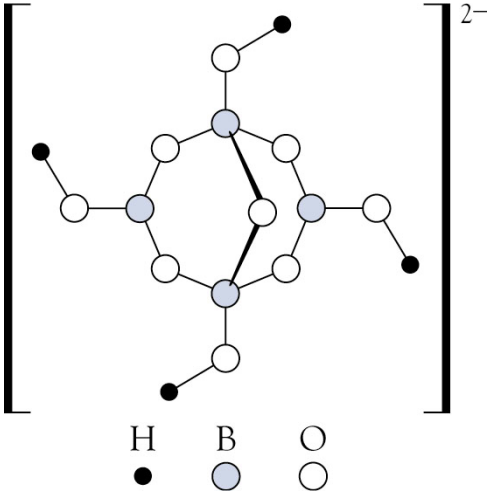
\includegraphics[width=0.5\textwidth]{figures/k13s293Borax.png}
\end{flashcard}

\begin{flashcard}[Struktur]{Tegn strukturen af peroxoborationen}
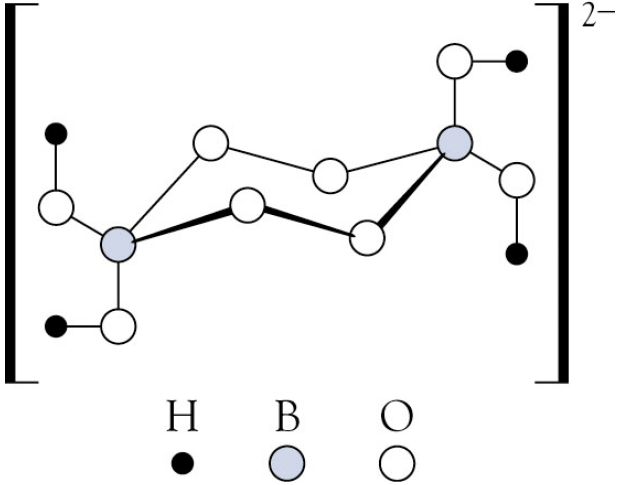
\includegraphics[width=0.5\textwidth]{figures/k13s293Peroxoborat.png}
\end{flashcard}

\begin{flashcard}[Fremstilling]{Opskriv reaktionen for fremstilling af peroxoborationen}
\ce{[B4O5(OH)4]^{2-} + 4H2O2 + 2OH- -> 2[B2(O2)2(OH)4]^{2-} + 3H2O}
\end{flashcard}

\begin{flashcard}[Fremstilling]{Opskriv reaktionen for fremstilling af borcarbid samt reaktionen for fremstilling af titaniumborid}
\ce{2B2O3 + 7C ->[\text{$\Delta$}] B4C + 6CO}\\ \vspace{7pt}
\ce{2TiO2 + B4C + 3C ->[\text{$\Delta$}] 2TiB2 + 4CO}
\end{flashcard}

\begin{flashcard}[Struktur]{Tegn strukturen af diboran}
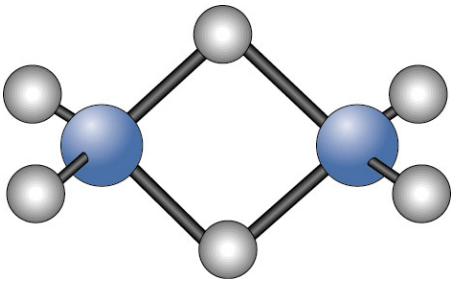
\includegraphics[width=0.5\textwidth]{figures/k13s295Diboran.png}
\end{flashcard}

\begin{flashcard}[Struktur]{Tegn strukturen af pentaboran(9)}
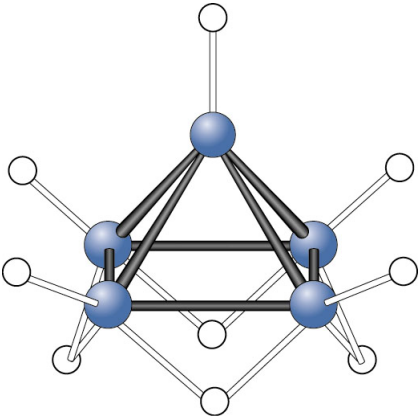
\includegraphics[width=0.5\textwidth]{figures/k13s296Pentaboran.png}
\end{flashcard}

\begin{flashcard}[Struktur]{Tegn strukturen af tetraboran(10)}
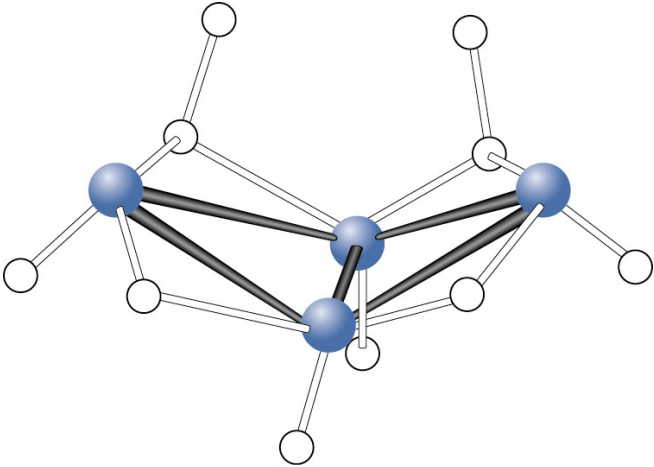
\includegraphics[width=0.7\textwidth]{figures/k13s296Tetraboran.png}
\end{flashcard}

\begin{flashcard}[Fremstilling]{Beskriv fremstillingen af diboran ved hjælp af et reaktionsskema}
\begin{align*}
\ce{2\OX{rf1,\ox{+3,\ce{B}}}F3 + 6Na\OX{of1,\ox{-1,\ce{H}}} -> \OX{re1,\ox{-3,\ce{B2}}}\OX{oe1,\ox{+1,\ce{H6}}} + 6NaF}
\redox(of1,oe1){\small oxidation}
\redox(rf1,re1)[][-1]{\small reduktion}
\end{align*}
\end{flashcard}

\begin{flashcard}[Fremstilling]{Beskriv fremstillingen af tetraboran og pentaboran med reaktionsskemaer}
\ce{2B2H6 -> B4H10 + H2} \\ \vspace{7pt}
\ce{B4H10 + B2H6 -> 2B5H11 + 2H2}
\end{flashcard}

\begin{flashcard}[Reaktion]{Opskriv diborans reaktion med oxygen og vand}
\ce{B2H6 + 3O2 -> B2O3 + 3H2O}\\ \vspace{7pt}
\ce{B2H6 + 6H2O -> 2H3BO3 +6H2}
\end{flashcard}

\begin{flashcard}[Fremstilling]{Opskriv reaktionen for fremstilling af natriumborhydrid}
\ce{B2H6 + 2NaH -> 2NaBH4}
\end{flashcard}

\begin{flashcard}[Egenskab]{Aluminium metal er amfotert. Opskriv dets reaktion med syre henholdsvis base}
\ce{2Al + 6H+ + 6H2O -> 2[Al(OH2)6]^{3+} + 3H2}\\ \vspace{7pt}
\ce{2Al + 2OH- + 6H2O -> 2[Al(OH)4]- + 3H2}
\end{flashcard}

\begin{flashcard}[Egenskab]{Aluminium(III) i vandig opløsning er en svag syre på linje med eddikesyre. Opskriv reaktionen med vand}
\ce{[Al(OH2)6]^{3+} + H2O -> [Al(OH2)5(OH)]^{2+} + H3O+}
\end{flashcard}

\begin{flashcard}[Fremstilling]{Beskriv den industrielle fremstilling af aluminium metal med reaktionsskemaer}
\ce{Al2O3 + 2OH- + 3H2O -> 2[Al(OH)4]-}\\
\ce{2[Al(OH)4]- -> Al2O3\cdot 3H2O(s) + 2OH-}\\
\ce{Al2O3\cdot 3H2O ->[\text{$\Delta$}] Al2O3 + 3H2O}\\
Herefter følger elektrolyse af smeltet aluminiumoxid i cryolit
\end{flashcard}

\begin{flashcard}[Fremstilling]{Beskriv den industrielle fremstilling af cryolit med reaktionsskemaer}
\ce{3SiF4 + 2H2O -> 2H2SiF6 + SiO2}\\
\ce{H2SiF6 + 6NH3 + 2H2O -> 6NH4F + SiO2}\\ \vspace{7pt}
\ce{6NH4F + Na[Al(OH)4] + 2NaOH -> Na3AlF6 + 6NH3 + 6H2O}
\end{flashcard}

\begin{flashcard}[Struktur]{Hvilken struktur har \ce{MgAl2O4} henholdsvis \ce{Fe3O4}?}
\ce{MgAl2O4} er en spinel mens \ce{Fe3O4} er en invers spinel
\end{flashcard}
%\cardfrontfoot{Kapitel 14}
\begin{flashcard}[Egenskab]{Opskriv 3 ioniske, 2 covalente og 2 metalliske carbider}
Ioniske: \ce{Na2C2}, \ce{Be2C} og \ce{Al4C3}\\ \vspace{7pt}
Covalente: \ce{SiC} og \ce{B4C}\\ \vspace{7pt}
Metalliske: \ce{WC} og \ce{Fe3C}
\end{flashcard}

\begin{flashcard}[Anvendelse]{Angiv en anvendelse af \ce{Na2C2}}
\ce{Na2C2 + 2H2O -> 2NaOH + C2H2}
\end{flashcard}

\begin{flashcard}[Fremstilling]{Angiv med reaktionsskema en metode til at fremstille carbonmonoxid i laboratoriet}
\ce{HCOOH + H2SO4(l) -> CO + H2O + H2SO4(aq)}
\end{flashcard}

\begin{flashcard}[Fremstilling]{Angiv med reaktionsskema hvordan man kan fremstille methanol og propanal ud fra bl.a. carbonmonoxid}
\ce{CO + 2H2 -> CH3OH} \\ \vspace{7pt}
\ce{CO + C2H4 + H2 -> C2H5CHO}
\end{flashcard}

\begin{flashcard}[Anvendelse]{Hvordan kan man undersøge om der er carbondioxid i en gasstrøm?}
Man kan lede strømmen gennem en opløsning af  \ce{Ba(OH)2} eller \ce{Ca(OH)2}. Testen er positiv hvis der opstår et bundfald.
\end{flashcard}

\begin{flashcard}[Reaktion]{Beskriv med reaktionsskema hvad der sker når man varmer følgende faste carbonater op:\\ \vspace{7pt}
\ce{CaCO3}, \ce{Ag2CO3}, \ce{(NH4)2CO3} og \ce{NaHCO3}
}
\ce{CaCO3 ->[\text{$\Delta$}] CaO + CO2}\\ \vspace{7pt}
\ce{Ag2CO3 ->[\text{$\Delta$}] Ag2O + CO2}\\
\ce{Ag2O ->[\text{$\Delta$}] 2Ag + $\frac{1}{2}$O2}\\ \vspace{7pt}
\ce{(NH4)2CO3 ->[\text{$\Delta$}] 2NH3 + H2O + CO2}\\ \vspace{7pt}
\ce{2NaHCO3 ->[\text{$\Delta$}] Na2CO3 + H2O + CO2}
\end{flashcard}

\begin{flashcard}[Fremstilling]{Beskriv med reaktionsskema hvordan man fremstiller carbondisulfid industrielt}
\ce{CH4 + 4S(l) ->[\text{$\Delta$}] CS2 + 2H2S}
\end{flashcard}

\begin{flashcard}[Fremstilling]{Opskriv to metoder til at producere \ce{CCl4}}
\begin{itemize}
\item \ce{CS2 + 3Cl2 ->[\text{$\rm FeCl_{3}/\Delta$}] CCl4 + S2Cl2}\\
\ce{CS2 + 2S2Cl2 ->[\text{$\Delta$}] CCl4 + 6S}
\item \ce{CH4 + 4Cl2 -> CCl4 + 4HCl}
 \end{itemize}
\end{flashcard}

\begin{flashcard}[Fremstilling]{Angiv to industrielle metoder til at fremstille blåsyre}
\ce{CH4 + NH3 ->[\text{$\rm Pt/1200\,^{\circ}{\rm C}$}] HCN + 3H2}\\ \vspace{7pt}
\ce{2CH4 + 2NH3 + 3O2 ->[\text{$\rm Pt/Rh/1100\,^{\circ}{\rm C}$}] 2HCN + 6H2O}
\end{flashcard}

\begin{flashcard}[Fremstilling]{Opskriv hvordan man fremstiller silicium industrielt}
\ce{SiO2 + 2C ->[\text{$\Delta$}] Si(l) + 2CO}
\end{flashcard}

\begin{flashcard}[Fremstilling]{Opskriv to metoder til at oprense silicium industrielt}
Følgende ligevægt kan bruges til at destillere silicium. Ligevægten er forskudt med højre ved ca $300\,^{\circ}{\rm C}$ og mod venstre ved $1000\,^{\circ}{\rm C}$.\\
\ce{Si + 3HCl <=> SiHCl3(g) + H2}\\ \vspace{7pt}
En alternativ metode er zone-refining:
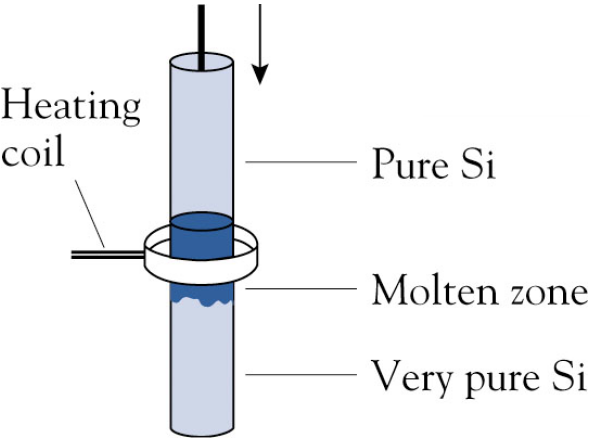
\includegraphics[width=0.37\textwidth]{figures/k14s340ZoneRefining.png}
\end{flashcard}

\begin{flashcard}[Reaktion]{Opskriv den kemiske formel for to kemikalier som kan reagere med glas samt deres reaktion}
Der er tale om \ce{HF} og \ce{NaOH}\\ \vspace{7pt}
\ce{SiO2 + 6HF -> SiF6^{2-} + 2H+ + 2H2O}\\ \vspace{7pt}
\ce{SiO2 + 2NaOH ->[\text{$\Delta$}] Na2SiO3 + H2O}
\end{flashcard}

\begin{flashcard}[Egenskab]{Opskriv de fire typer glas der er omtalt i bogen og angiv fordele ved hver af dem}
\begin{itemize}
\item Soda-lime\\Billigt
\item Borosilicate\\Kan klare store temperaturudsving
\item Lead\\Absorberer radioaktiv stråling
\item Quartz\\Er også gennemsigtigt i UV området
\end{itemize}
\end{flashcard}

\begin{flashcard}[Fremstilling]{Angiv med reaktionsskema hvordan man kan fremstille natriumsilicat}
\ce{SiO2 + 2Na2CO3(l) ->[\text{$\Delta$}] Na4SiO4 + 2CO2}
\end{flashcard}

\begin{flashcard}[Struktur]{Tegn strukturen af pyrosilicationen}
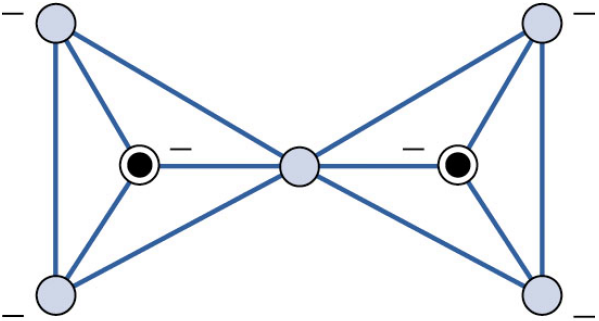
\includegraphics[width=0.5\textwidth]{figures/k14s344Pyrosilicate.png}
\end{flashcard}

\begin{flashcard}[Reaktion]{Angiv reaktionen mellem silicationen og syre}
\ce{2SiO4^{4-} + 2H+ -> Si2O7^{6-} + H2O}
\end{flashcard}

\begin{flashcard}[Struktur]{Angiv de kemiske formler for hvid og blå asbest og angiv hvilken der er farligst}
Hvid asbest: \ce{Mg3(Si2O5)(OH)4}\\ \vspace{7pt}

Blå asbest: \ce{Na2Fe5(Si4O11)2(OH)2} (farligst)
\end{flashcard}

\begin{flashcard}[Fremstilling]{Angiv hvordan silikone laves ved hjælp af reaktionsskemaer samt strukturen af silikone}
\ce{2CH3Cl + Si ->[\text{$\Delta$}] (CH3)2SiCl2}\\
\ce{(CH3)2SiCl2 + 2H2O -> (CH3)2(Si(OH)2 + 2HCl}\\
\ce{$n$(CH3)2Si(OH)2 -> [-O-Si(CH3)2-]_{$n$} + H2O}\\ \vspace{7pt}
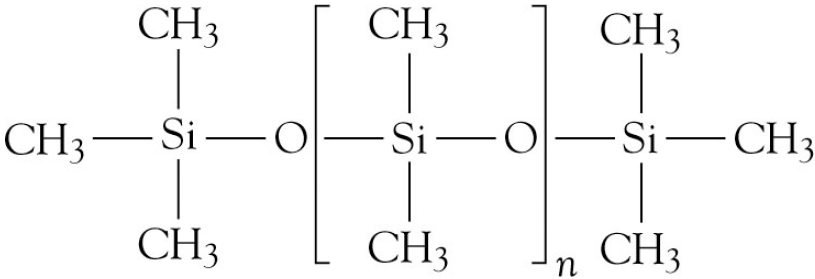
\includegraphics[width=0.9\textwidth]{figures/k14s349Silikone.png}
\end{flashcard}

\begin{flashcard}[Reaktion]{Angiv tin(II)oxids reaktion med syre henholdsvis base}
\ce{SnO + 2HCl -> SnCl2 + H2O}\\ \vspace{7pt}
\ce{SnO + NaOH + H2O -> Na+ + [Sn(OH)3]-}
\end{flashcard}

\begin{flashcard}[Fremstilling]{Angiv den primære kilde af bly i naturen samt hvordan man udvinder bly fra denne}
Den primære naturlige kilde er \ce{PbS}\\ \vspace{7pt}
\ce{2PbS + 3O2 ->[\text{$\Delta$}] 2PbO + 2SO2}\\
\ce{PbO + C ->[\text{$\Delta$}] Pb + CO}
\end{flashcard}

\begin{flashcard}[Reaktion]{Angiv med reaktionsskema hvorledes \ce{PbCl4} dekomponerer}
\begin{align*}
\ce{\OX{rf1,\ox{+4,\ce{Pb}}}\OX{of1,\ox{-1,\ce{Cl4}}} -> \OX{re1,\ox{2,\ce{Pb}}} Cl2 + \OX{oe1,\ox{0,\ce{Cl2}}}}
\redox(of1,oe1){\small oxidation}
\redox(rf1,re1)[][-1]{\small reduktion}
\end{align*}
\end{flashcard}
%\cardfrontfoot{Kapitel 15}

\begin{flashcard}[Egenskab]{Hvordan fremstår grundstofferne i 5. hovedgruppe ved SATP?}
Nitrogen er en farveløs gas. Fosfor er en hvis voks-agtig substans. De resterende er skrøblige metaller.
\end{flashcard}

\begin{flashcard}[Teori]{Angiv de specier der har tendens til at disproportionere i sur opløsning\\
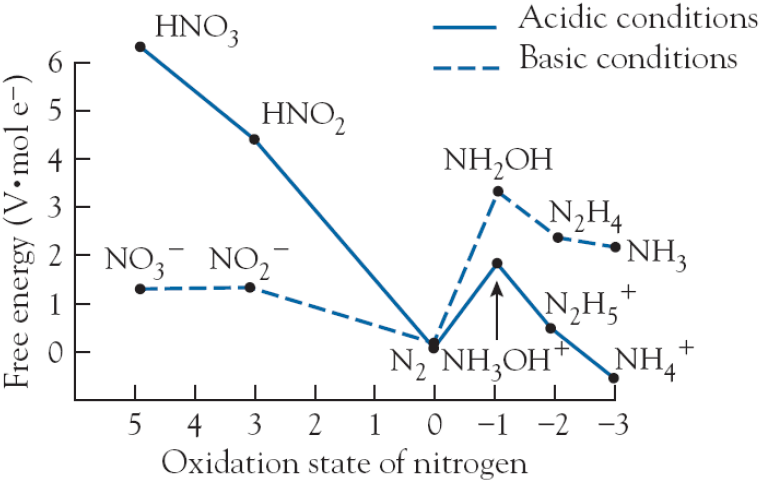
\includegraphics[width=0.55\textwidth]{figures/k15s368FrostDiagram.png}
}
\ce{HNO2} samt \ce{NH3OH+}
\end{flashcard}

\begin{flashcard}[Fremstilling]{Angiv hvordan ammoniak kan fremstilles i laboratoriet}
\ce{NH4Cl + NaOH -> NH3(g) + NaCl}
\end{flashcard}

\begin{flashcard}[Fremstilling]{Opskriv hvordan ammoniak fremstilles industrielt}
\ce{CH4 + H2O -> CO + 3H2}\\
\ce{ZnO + H2S -> ZnS + 2H2O}\\
\ce{Ch4 + $\frac{1}{2}$O2 + 2N2 -> CO + 2H2 + 2N2}\\
\ce{CO + H2O <=> CO + H2}\\
\ce{CO2 + K2CO3 + H2O <=> 2KHCO3}\\
\ce{ N_{2} + 3H_{2} <=> 2NH_{3}}\\ \vspace{7pt}
ved et tryk på 100-1000 atm og en temperatur på 400-500$\,^{\circ}{\rm C}$
\end{flashcard}

\begin{flashcard}[Egenskab]{Reagerer hydrazin alkalisk eller neutralt?}
Alkalisk\\ \vspace{7pt}
\ce{N2H4 + H3O+ -> N2H5+ + H2O}
\end{flashcard}

\begin{flashcard}[Egenskab]{Angiv hvordan hydrazin kan anvendes som reduktionsmiddel}
\ce{N2H4 + 2I2 -> 4HI + N2}\\ \vspace{7pt}
\ce{N2H4 + 2Cu^{2+} -> 2Cu + N2 + 4H+}
\end{flashcard}

\begin{flashcard}[Struktur]{Tegn hydrazin}
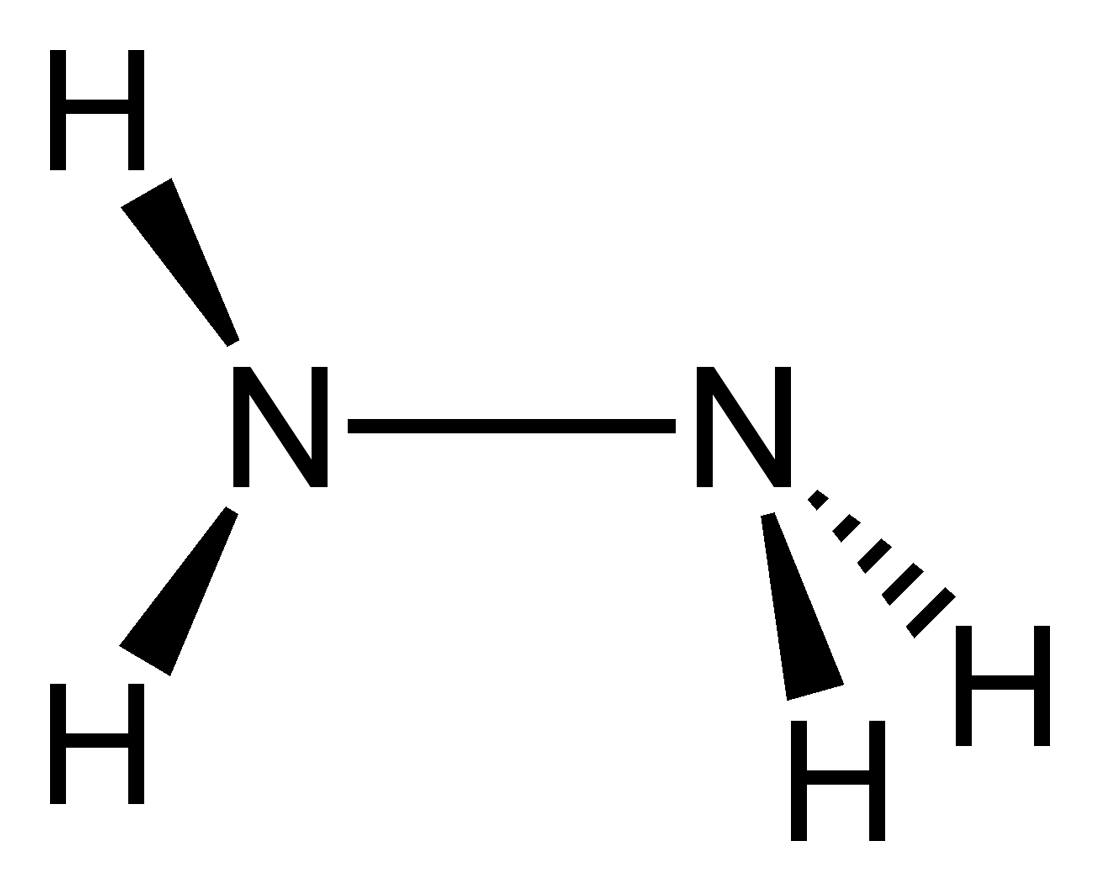
\includegraphics[width=0.55\textwidth]{figures/Hydrazin.png}
\end{flashcard}

\begin{flashcard}[Reaktion]{Angiv hvordan hydrogenazid dekomponerer}
\ce{2HN3 -> H2 + 3N2}
\end{flashcard}

\begin{flashcard}[Anvendelse]{Forklar hvordan en airbag virker ved hjælp af reaktionsligninger}
\ce{2NaN3 ->[\text{$\Delta$}] 2Na(l) + 3N2}\\
\ce{10Na(l) + 2KNO3 -> K2O + 5Na2O + N2}\\
\ce{2K2O + SiO2 -> K4SiO4}\\
\ce{2Na2O + SiO2 -> Na4SiO4}
\end{flashcard}

\begin{flashcard}[Reaktion]{Angiv hvordan følgende forbindelser dekomponerer ved opvarmning\\
\ce{NH4NO2}, \ce{NH4NO3} samt \ce{(NH4)2Cr2O7}
}
\ce{NH4NO2 ->[\text{$\Delta$}] N2 + 2H2O}\\ \vspace{7pt}
\ce{NH4NO3 ->[\text{$\Delta$}] N2O + 2H2O}\\ \vspace{7pt}
\ce{(NH4)2Cr2O7 ->[\text{$\Delta$}] N2 + Cr2O3 + 4H2O}
\end{flashcard}

\begin{flashcard}[Reaktion]{Angiv en metode til at producere lattergas}
\ce{NH4NO3 ->[\ce{H+}] N2O + 2H2O}
\end{flashcard}

\begin{flashcard}[Reaktion]{Angiv en metode til at producere nitrogenmonoxid}
\ce{3Cu + 8HNO3 -> 3Cu(NO3)2 + 4H2O + 2NO}
\end{flashcard}

\begin{flashcard}[Reaktion]{Angiv en metode til at producere \ce{N2O3}}
\ce{NO + NO2 -> N2O3(l)}
\end{flashcard}

\begin{flashcard}[Reaktion]{Angiv reaktionen mellem \ce{N2O3} og vand}
\ce{N2O3 + H2O -> 2HNO2}
\end{flashcard}

\begin{flashcard}[Struktur]{Tegn dinitrogentrioxid}
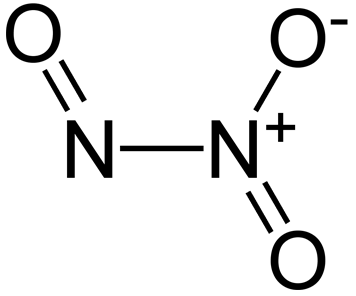
\includegraphics[width=0.55\textwidth]{figures/Dinitrogentrioxid.png}
\end{flashcard}

\begin{flashcard}[Reaktion]{Angiv to metoder til at producere nitrogendioxid}
\ce{Cu + 4HNO3 -> Cu(NO3)2 + 2H2O + 2NO2}\\ \vspace{7pt}
\ce{Cu(NO3)2 ->[\text{$\Delta$}] CuO + 2NO2 + $\frac{1}{2}$O2}
\end{flashcard}

\begin{flashcard}[Reaktion]{Angiv reaktionen mellem nitrogendioxid og vand}
\ce{2NO2 + H2O <=> HNO3 + HNO2}
\end{flashcard}

\begin{flashcard}[Struktur]{Tegn nitrogendioxid}
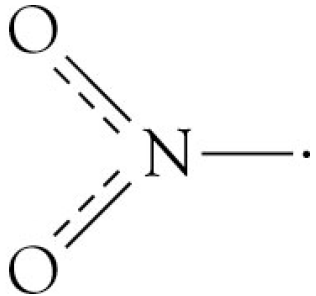
\includegraphics[width=0.3\textwidth]{figures/k15s383Nitrogendioxid.png}
\end{flashcard}

\begin{flashcard}[Struktur]{Tegn dinitrogentetroxid}
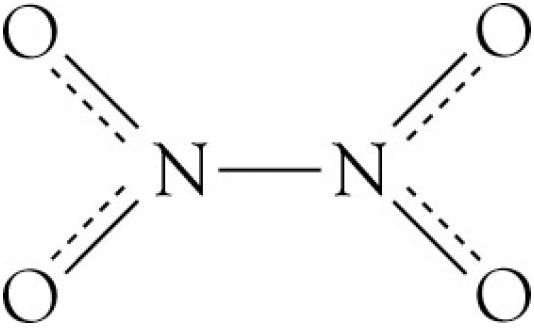
\includegraphics[width=0.5\textwidth]{figures/k15s383Dinitrogentetroxid.png}
\end{flashcard}

\begin{flashcard}[Struktur]{Tegn dinitrogenpentoxid}
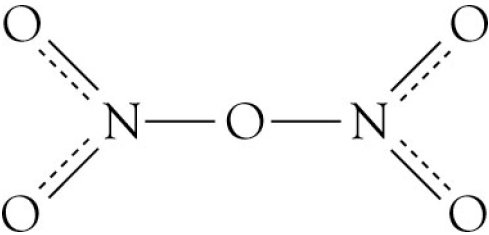
\includegraphics[width=0.5\textwidth]{figures/k15s383Dinitrogenpentoxid.png}
\end{flashcard}

\begin{flashcard}[Struktur]{Tegn nitrat}
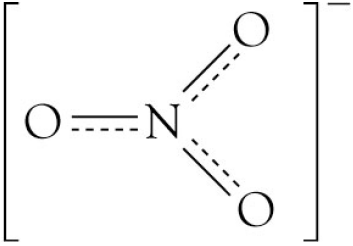
\includegraphics[width=0.5\textwidth]{figures/k15s383Nitrat.png}
\end{flashcard}

\begin{flashcard}[Struktur]{Tegn nitrit}
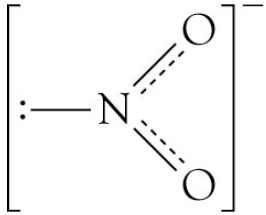
\includegraphics[width=0.5\textwidth]{figures/k15s385Nitrit.png}
\end{flashcard}

\begin{flashcard}[Fremstilling]{Angiv med reaktionsligning hvordan man kan fremstille salpetersyrling i laboratoriet}
\ce{Ba(NO2)2 + H2SO4 -> BaSO4(s) + 2HNO2}
\end{flashcard}

\begin{flashcard}[Reaktion]{Angiv med reaktionsligning hvordan salpetersyrling disproportionerer}
\begin{align*}
\ce{3H\OX{d,\ox{+3,\ce{N}}}O2 -> H\OX{oe1,\ox{5,\ce{N}}}O3 + 2\OX{re1,\ox{+2,\ce{N}}}O}
\redox(d,oe1){\small oxidation}
\redox(d,re1)[][-1]{\small reduktion}
\end{align*}\\ \vspace{15pt}
(\ce{2NO + O2 -> 2NO2})
\end{flashcard}

\begin{flashcard}[Fremstilling]{Opskriv hvordan man producerer salpetersyre industrielt via. Ostwald-processen}
\ce{4NH3 + 5O2 -> 4NO + 6H2O}\\
\ce{2NO + O2 -> 2NO2}\\
\ce{3NO2 + H2O -> 2HNO3 + NO}
\end{flashcard}

\begin{flashcard}[Anvendelse]{Angiv den eksoterme reaktion der finder sted i en cold pack}
\ce{NH4NO3(s) -> NH4+ + NO3-}
\end{flashcard}

\begin{flashcard}[Struktur]{Tegn strukturen af hvid henholdsvis rød fosfor}
Hvid:\\
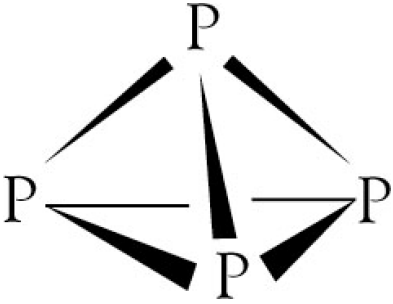
\includegraphics[width=0.2\textwidth]{figures/k15s390HvidP.png}\\
Rød:\\
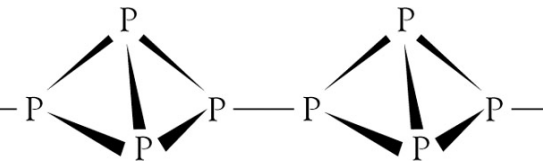
\includegraphics[width=0.6\textwidth]{figures/k15s390RodP.png}
\end{flashcard}

\begin{flashcard}[Reaktion]{Hvad sker der med hvid fosfor der udsættes for UV lys?}
Det omdannes til dens allotrop, rød fosfor
\end{flashcard}

\begin{flashcard}[Reaktion]{Hvorfor skal hvid fosfor opbevares under vand?}
Fordi det reagerer med atmosfærens oxygen\\
\ce{P4 + 5O2 -> P4O10}
\end{flashcard}

\begin{flashcard}[Fremstilling]{Hvordan udvindes fosfor industrielt?}
\ce{2Ca3(PO4)2 + 10CO ->[\text{$\Delta$}] 6CaO + 10CO2 + P4(g)}\\
\ce{CO2 + C -> 2CO} \\
\ce{CaO + SiO2 ->[\text{$\Delta$}] CaSiO3(l)}\\ \vspace{7pt}
Reaktionerne foregår ved $\rm 1500\,^{\circ}{\rm C}$.
\end{flashcard}

\begin{flashcard}[Fremstilling]{Hvordan fremstilles phosphin?}
\ce{Ca3P2 + 6H2O(s) -> 2PH3 + 3Ca(OH)2}
\end{flashcard}

\begin{flashcard}[Reaktion]{Opskriv reaktionerne hvorved de to oxider af fosfor dannes}
\ce{P4 + 3O2 -> P4O6}\\ \vspace{7pt}
\ce{P4 + 5O2 -> P4O10}
\end{flashcard}

\begin{flashcard}[Struktur]{Tegn strukturen af \ce{P4O6}}
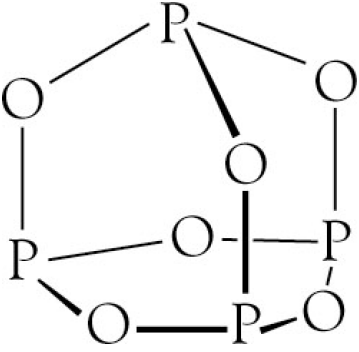
\includegraphics[width=0.4\textwidth]{figures/k15s393P4O6.png}
\end{flashcard}

\begin{flashcard}[Struktur]{Tegn strukturen af \ce{P4O10}}
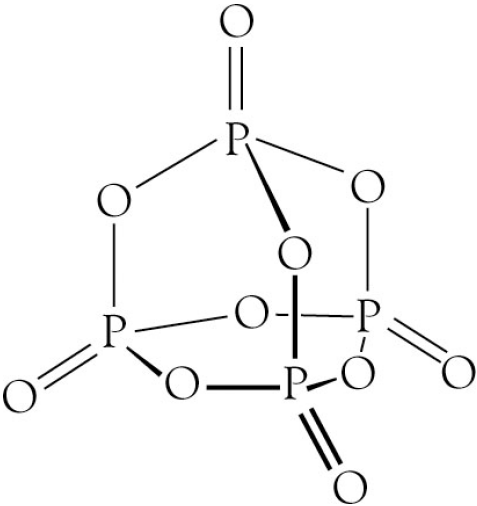
\includegraphics[width=0.4\textwidth]{figures/k15s394P4O10.png}
\end{flashcard}

\begin{flashcard}[Reaktion]{Angiv reaktionen mellem \ce{P4O10} og vand}
\ce{P4O10 + 6H2O + 4H3PO4}
\end{flashcard}

\begin{flashcard}[Reaktion]{Opskriv reaktionligninger for hvordan man danner de to chlorider af fosfor}
\ce{P4 + 6Cl2 -> 4PCl3}\\ \vspace{7pt}
\ce{P4 + 10Cl2 -> 4PCl5}
\end{flashcard}

\begin{flashcard}[Reaktion]{Angiv phosphortrichlorids henholdsvis phosphorpentachlorids reaktion med vand}
\ce{PCl3 + H2O -> H3PO3 + 3HCl}\\ \vspace{7pt}
\ce{PCl5 + H2O -> POCl3 + 2HCl}\\
\ce{POCl3 + 3H2O -> H3PO4 + 3HCl}
\end{flashcard}

\begin{flashcard}[Fremstilling]{Angiv med reaktionsskema hvorledes \ce{POCl3} fremstilles}
\ce{2PCl3 + O2 -> 2POCl3}
\end{flashcard}

\begin{flashcard}[Struktur]{Tegn \ce{H3PO4}, \ce{H3PO3} samt \ce{H3PO2}}
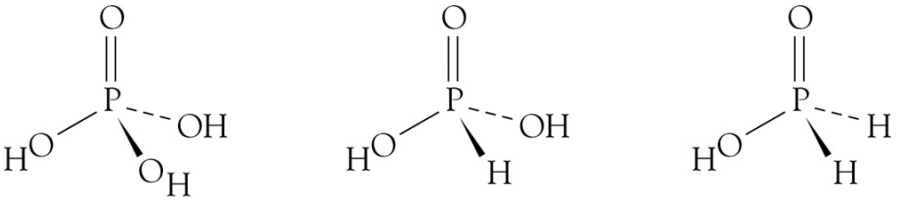
\includegraphics[width=0.9\textwidth]{figures/k15s395POxyAcids.png}
\end{flashcard}

\begin{flashcard}[Fremstilling]{Angiv hvordan fosforsyre fremstilles ved vådprocessen}
\ce{Ca3(PO4)2 + 3H2SO4 -> 3CaSO4(s) + 2H3PO4}
\end{flashcard}

\begin{flashcard}[Struktur]{Angiv strukturen af kondensationsproduktet der fås ved opvarmning af fosforsyre}
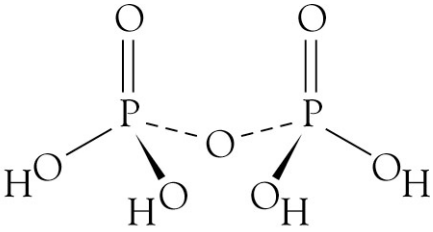
\includegraphics[width=0.6\textwidth]{figures/k15s396H4P2O7.png}
\end{flashcard}

\begin{flashcard}[Fremstilling]{Angiv med reaktionsskema hvordan calciumfosfat kan bearbejdes så det kan bruges som gødning}
\ce{Ca3(PO4)2(s) + 2H2SO4 -> Ca(H2PO4)2(s) + 2CaSO4(s)}
\end{flashcard}
%\cardfrontfoot{Kapitel 16}

\begin{flashcard}[Fremstilling]{Angiv 2 metoder til at fremstille oxygen i laboratoriet}
\ce{2KClO3 ->[\text{$\rm MnO2/\Delta$}] 2KCl + 3O2}\\ \vspace{7pt}
\ce{2H2O2 ->[\text{$\rm MnO2$}] 2H2O + O2}
\end{flashcard}

\begin{flashcard}[Fremstilling]{Angiv hvordan man kan fremstille diamagnetisk \ce{O2}}
\ce{H2O2 + ClO- -> O2 + H2O + Cl-}
\end{flashcard}

\begin{flashcard}[Fremstilling]{Angiv hvordan man kan fremstille ozon}
\ce{3O2 -> 2O3}\\
ved påføring af en spænding på 10-20kV
\end{flashcard}

\begin{flashcard}[Reaktion]{Angiv produktet af reaktion mellem følgende forbindelser og ozon: \ce{NO2}, \ce{CN-} samt \ce{PbS}}
\ce{2NO2 + O3 -> N2O5 + O2} \\ \vspace{7pt}
\ce{CN- + O3 -> OCN- + O2} \\ \vspace{7pt}
\ce{PbS + 4O3 -> PbSO4 + 4O2}
\end{flashcard}

\begin{flashcard}[Egenskab]{Kategoriser disse metaloxider som enten: meget basiske, basiske, amfotere eller sure\\
\ce{Na2O}, \ce{CaO}, \ce{MnO}, \ce{Al2O3}, \ce{Cr2O3}, \ce{SnO2}, \ce{V2O5}, \ce{CrO3} samt \ce{Mn2O7}
}
Meget basisk: \ce{Na2O}\\
Basisk: \ce{CaO} og \ce{MnO}\\
Amfoter: \ce{Al2O3}, \ce{Cr2O3}, \ce{SnO2} og \ce{V2O5}\\
Sure: \ce{CrO3} og \ce{Mn2O7}
\end{flashcard}

\begin{flashcard}[Egenskab]{Kategoriser disse ikke-metaloxider som enten: neutrale, sure eller meget sure\\
\ce{N2O}, \ce{CO}, \ce{N2O3}, \ce{NO2}, \ce{CO2}, \ce{SO2}, \ce{N2O5}, \ce{SO3} samt \ce{Cl2O7}
}
Neutrale: \ce{N2O} og \ce{CO}\\
Sure: \ce{N2O3}, \ce{NO2}, \ce{CO2} og \ce{SO2}\\
Meget sure: \ce{N2O5}, \ce{SO3} og \ce{Cl2O7}
\end{flashcard}

\begin{flashcard}[Fremstilling]{Angiv hvordan hydrogenperoxid kan fremstilles i laboratoriet}
\ce{Na2O2 + 2H2O -> 2NaOH + H2O2}
\end{flashcard}

\begin{flashcard}[Egenskab]{Hydrogenperoxid har tendens til at disproportionere. Opskriv reaktionen}
\ce{2H2O2 -> 2H2O + O2}
\end{flashcard}

\begin{flashcard}[Struktur]{Tegn strukturen af \ce{S6}}
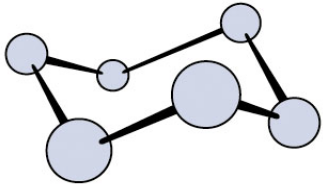
\includegraphics[width=0.6\textwidth]{figures/k16s428S6.png}
\end{flashcard}

\begin{flashcard}[Struktur]{Tegn strukturen af \ce{S8}}
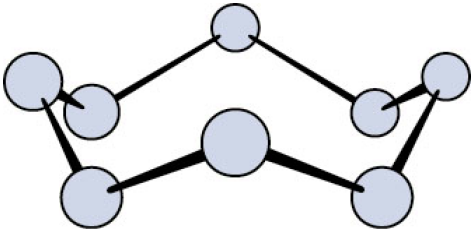
\includegraphics[width=0.6\textwidth]{figures/k16s427S8.png}
\end{flashcard}

\begin{flashcard}[Struktur]{Tegn strukturen af \ce{S12}}
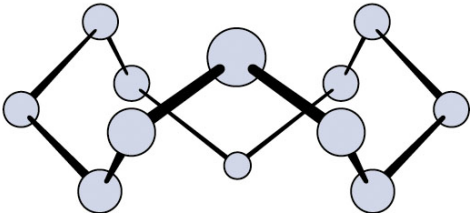
\includegraphics[width=0.7\textwidth]{figures/k16s428S12.png}
\end{flashcard}

\begin{flashcard}[Fremstilling]{Opskriv hvordan man kan fremstille \ce{S6}}
\ce{6Na2S2O3 + 12HCl -> S6(s) + 6SO2 + 12NaCl + 6H2O}
\end{flashcard}

\begin{flashcard}[Fremstilling]{Opskriv hvordan man kan fremstille \ce{S12}}
\ce{H2S8 + S4Cl2 -> S12(s) + 2HCl(g)}
\end{flashcard}

\begin{flashcard}[Fremstilling]{Opskriv reaktionsligninger der beskriver Claus processen}
\ce{2H2S + 3O2 -> 2SO2 + 2H2O}\\
\ce{4H2S + 2SO2 -> 6S(s) + 4H2O}
\end{flashcard}

\begin{flashcard}[Fremstilling]{Angiv hvordan man kan udvinde svovl fra pyrit}
\ce{FeS2 ->[\text{$\Delta$}] FeS + S(s)}
\end{flashcard}

\begin{flashcard}[Reaktion]{Hvordan kan man påvise sulfid i en vandig opløsning?}
\ce{Pb(CH3COO)2 + H2S(g) -> PbS + 2CH3COOH}\\ \vspace{7pt}
Blyacetat er farveløst. Ved reaktion fremkommer sort bly(II)sulfid
\end{flashcard}

\begin{flashcard}[Reaktion]{Hvordan kan man påvise \ce{SO2} i en vandig opløsning?}
\ce{Cr2O7^{2-} + 3SO2 + 2H+ -> 2Cr^{3+} + 3SO4^{2-} + H2O}\\ \vspace{7pt}
Dichromat er orange/gult. Ved reaktion skifter opløsningen farve til grøn pga. chrom(III) ioner
\end{flashcard}

\begin{flashcard}[Reaktion]{Hvordan kan kraftværker oplagre \ce{SO2}?}
\ce{2CaO + 2SO2 + O2 ->[\text{$\Delta$}] 2CaSO4}
\end{flashcard}

\begin{flashcard}[Fremstilling]{Opskriv reaktionsligninger der beskriver trinnene i den industrielle syntese af svovlsyre}
\ce{S + O2 ->[\text{$\Delta$}] SO2}\\
\ce{2SO2 + O2 ->[\text{$\rm V_{2}O_{5}/\Delta$}] 2SO3}\\
\ce{SO3 + H2SO4 -> H2S2O7}\\
\ce{H2S2O7 + H2O -> 2H2SO4}
\end{flashcard}

\begin{flashcard}[Struktur]{Tegn strukturen af \ce{H2SO4}}
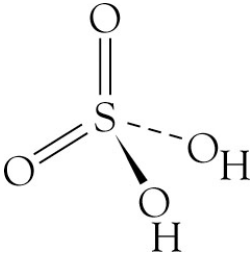
\includegraphics[width=0.4\textwidth]{figures/k16s438H2SO4.png}
\end{flashcard}

\begin{flashcard}[Struktur]{Tegn strukturen af \ce{H2S2O7}}
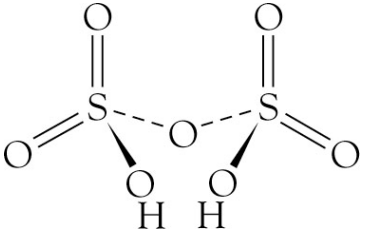
\includegraphics[width=0.7\textwidth]{figures/k16s439H2S2O7.png}
\end{flashcard}

\begin{flashcard}[Reaktion]{Hvad sker der hvis man varmer svovlsyre?}
\ce{2H2SO4 ->[\text{$\Delta$}] 2SO2 + 2H2O + O2}
\end{flashcard}

\begin{flashcard}[Fremstilling]{Angiv hvordan man kan fremstille thiosulfationen}
\ce{SO3^{2-} + S -> S2O3^{2-}}
\end{flashcard}

\begin{flashcard}[Struktur]{Tegn thiosulfationen}
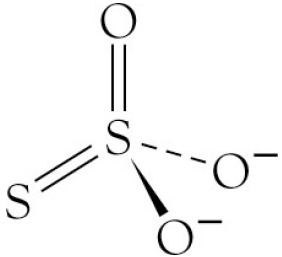
\includegraphics[width=0.5\textwidth]{figures/k16s442S2O32-.png}
\end{flashcard}

\begin{flashcard}[Struktur]{Tegn produktet af elektrolytisk oxidation af thiosulfationen}
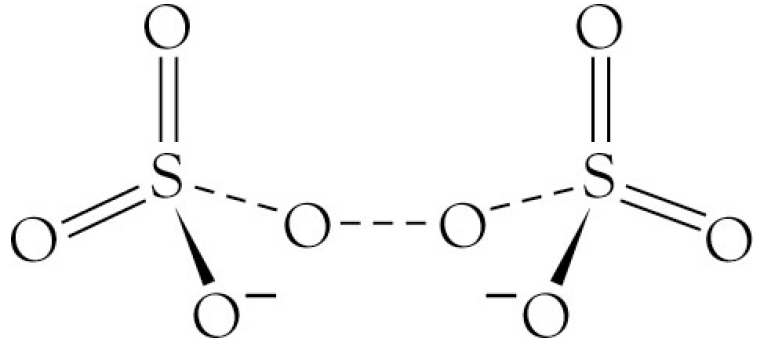
\includegraphics[width=0.7\textwidth]{figures/k16s443Peroxodisulfat.png}
\end{flashcard}

\begin{flashcard}[Fremstilling]{Angiv den simple reaktion for fremstilling af den inerte gas \ce{SF6}}
\ce{S(l) + 3F2(g) -> SF6(g)}
\end{flashcard}

\begin{flashcard}[Struktur]{Tegn strukturen af \ce{S2Cl2}}
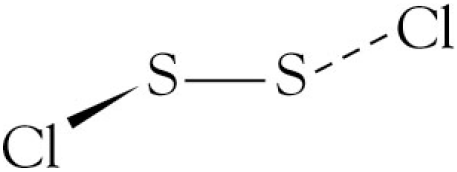
\includegraphics[width=0.7\textwidth]{figures/k16s444S2Cl2.png}
\end{flashcard}
%\cardfrontfoot{Kapitel 17}

\begin{flashcard}[Egenskab]{Hvordan fremstår halogenerne ved SATP?}
\ce{F2} fremstår som en bleg gul gas og \ce{Cl2} som en bleg grøn gas. \ce{Br2} er en rødbrun viskøs væske. Iod fremstår som glimtende sort-violette krystaller.
\end{flashcard}

\begin{flashcard}[Fremstilling]{Hvordan fremstilles \ce{F2}?}
Elektrolyse af kaliumfluorid
\end{flashcard}

\begin{flashcard}[Fremstilling]{Hvordan fremstilles \ce{UF6} industrielt?}
\ce{UO2 + 4HF -> UF4(s) + 2H2O}\\
\ce{UF4(s) + F2 -> UF6(g)}
\end{flashcard}

\begin{flashcard}[Fremstilling]{Hvordan produceres flussyre industrielt?}
\ce{CaF2 + H2SO4 -> 2HF(g) + CaSO4}
\end{flashcard}

\begin{flashcard}[Fremstilling]{Hvordan kan man fremstille chlorgas i laboratoriet og i industrien?}
I laboratoriet kan man nøjes med følgende\\
\ce{10HCl + 2MnO4- + 6H+ -> 5Cl2 + 2Mn^{2+} + 8H2O}\\ \vspace{7pt}
Industrielt produceres chlorgas som biprodukt ved elektrolyse af eksempelvis natriumchlorid opløsning med henblik på at producere natriummetal.
\end{flashcard}

\begin{flashcard}[Reaktion]{Angiv reaktionen mellem \ce{Cl2} og vand}
\ce{Cl2 + H2O -> H+ + Cl- + HClO}
\end{flashcard}

\begin{flashcard}[Fremstilling]{Hvordan fremstilles saltsyre industrielt?}
Saltsyre produceres hovedsagligt som biprodukt af andre synteser. Eksempelvis:\\
\ce{CH4 + 4Cl2 -> CCl4 + 4 HCl}
\end{flashcard}

\begin{flashcard}[Reaktion]{Hvordan fremstiller man jern(II)chlorid henholdsvis jern(III)chlorid?}
\ce{Fe + 2HCl -> FeCl2 + H2}\\ \vspace{7pt}
\ce{2Fe + 3Cl2 -> 2FeCl3}
\end{flashcard}

\begin{flashcard}[Reaktion]{Et af de 3 tungtopløselige sølvhalider går i opløsning ved tilsætning af ammoniak. Hvilket?}
Chlorid\\ \vspace{7pt}
\ce{AgCl(s) + 2NH3 -> [Ag(NH3)2]+ + Cl-}
\end{flashcard}

\begin{flashcard}[Struktur]{Angiv struktueren af følgende forbindelser: Hypochlorsyrling, chlorsyrling, chlorsyre og perchlorsyre}
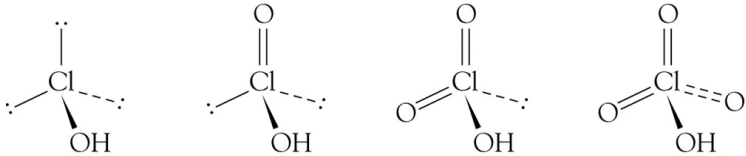
\includegraphics[width=\textwidth]{figures/k17s471Cl.png}
\end{flashcard}

\begin{flashcard}[Reaktion]{Angiv den reaktion der finder sted når chlorgas opløses i vand}
\ce{Cl2 + H2O <=> H+ + Cl- + HClO}
\end{flashcard}

\begin{flashcard}[Fremstilling]{Hvordan fremstilles perchlorat?}
\ce{3Cl2 + 6NaOH -> NaClO3 + 5NaCl(s) + 3H2O}\\ \vspace{7pt}
\ce{4KClO3(l) ->[\text{$\Delta$}] KCl(s) + 3KClO4(s)}
\end{flashcard}

\begin{flashcard}[Anvendelse]{Angiv reaktionen der finder sted når en faststof løfteraket affyres}
\ce{6NH4ClO4 + 8Al -> 4Al2O3 + 3N2 + 3Cl2 + 12H2O(g)}
\end{flashcard}
%\cardfrontfoot{Kapitel 18}

\begin{flashcard}[Struktur]{Tegn \ce{XeF2}, \ce{XeF4} og \ce{XeF6}}
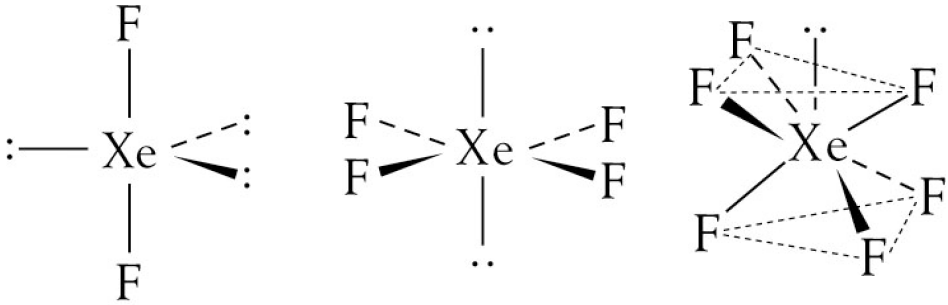
\includegraphics[width=1\textwidth]{figures/k18s493XeF.png}
\end{flashcard}

\begin{flashcard}[Struktur]{Tegn \ce{XeO3} og \ce{XeO4}}
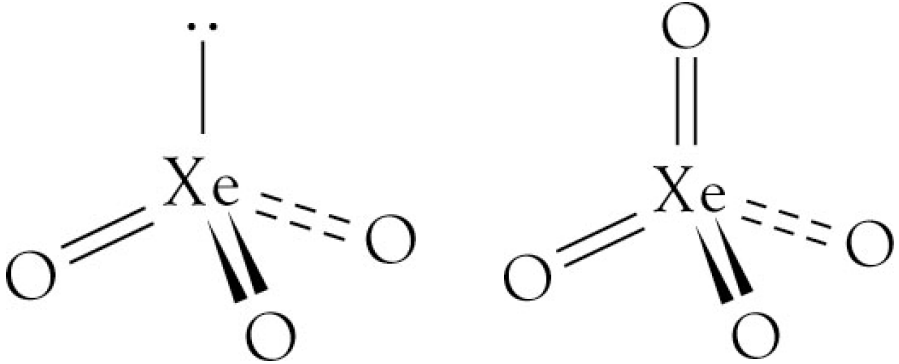
\includegraphics[width=0.8\textwidth]{figures/k18s494XeO.png}
\end{flashcard}
\cardfrontfoot{Kapitel 19}

\begin{flashcard}[Teori]{Hvad vil det sige at en ligang er mono-, bi-, etc. dentat?}
En monodentat ligand binder ved at donere et lonepair, en bidentat med to, tetradentat med fire osv.. Oxalat ionen er et eksempel på en chelat ligand.
\end{flashcard}

\begin{flashcard}[Struktur]{Tegn strukturen af ethylendiamintetraacetat $(\rm edta)^{4-}$ ionen}
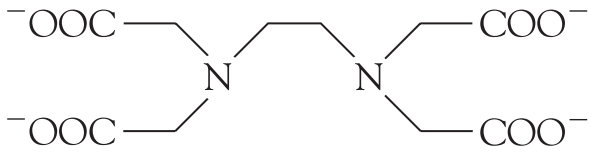
\includegraphics[width=0.8\textwidth]{figures/k19s503edta.png}
\end{flashcard}

\begin{flashcard}[Teori]{Vis med et eksempel hvad der forstås ved \textit{linkage isomerism}}
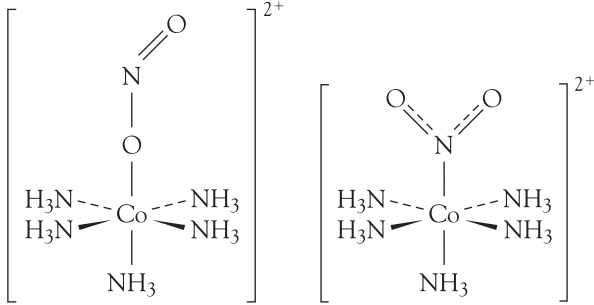
\includegraphics[width=0.8\textwidth]{figures/k19s504linkageisomerism.png}\\\vspace*{0.7cm}
hhv. \ce{[Co(ONO)(NH3)5]^{2+}} og \ce{[Co(NO2)(NH3)5]^{2+}} ionen
\end{flashcard}

\begin{flashcard}[Teori]{\ce{Co(NH3)5Br(SO4)} optræder i flere former. En af disse indeholder \ce{[CoBr(NH3)5]^{2+}} ionen mens en anden indeholder \ce{[CoSO4(NH3)5]^{+}} ionen. Hvilken slags isomeri er dette et eksempel på?}
Ion isomeri
\end{flashcard}

\begin{flashcard}[Teori]{Forklar med et eksempel hvad der forstås ved hydratiseringsisomeri}
Forbindelser der indeholder forskellige mængder krystalvand.
Ex. \ce{CrCl3*6H2O}, \ce{[CrCl(OH2)5]Cl2*H2O} og \ce{[CrCl2(OH2)4]Cl*2H2O}
\end{flashcard}

\begin{flashcard}[Teori]{Vis med et eksempel hvad der forstås ved koordinationsisomeri}
Når en forbindelse bestående af minimum to komplekser bytter ligander hvilket leder til en ny forbindelse. Ex. \ce{[Cr(NH3)6][Co(CN)6]} og \ce{[Co(NH3)6][Co(CN)6]}
\end{flashcard}

\begin{flashcard}[Teori]{Tegn de mulige stereoismere af et plankvadratisk kompleks}
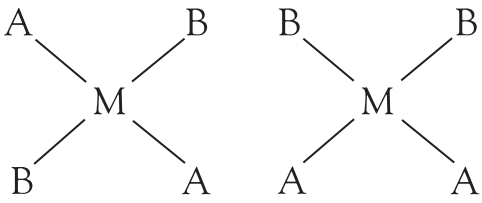
\includegraphics[width=0.8\textwidth]{figures/k19s505kvadisomere.png}
\end{flashcard}

\begin{flashcard}[Teori]{Tegn de mulige stereoismere af et oktaederisk kompleks}
\vspace*{-0.2cm}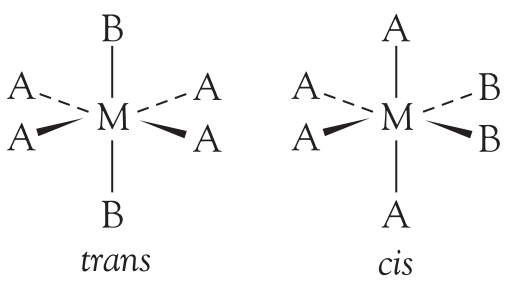
\includegraphics[width=0.5\textwidth]{figures/k19s505hexcistrans.png}\vspace*{0.5cm}
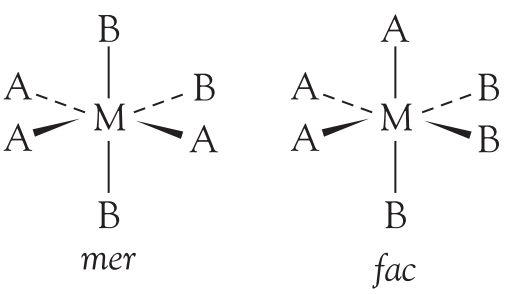
\includegraphics[width=0.5\textwidth]{figures/k19s506hexmerfac.png}
\end{flashcard}

\begin{flashcard}[Teori]{Giv et eksempel på hvordan et chiralt kompleks kan se ud}
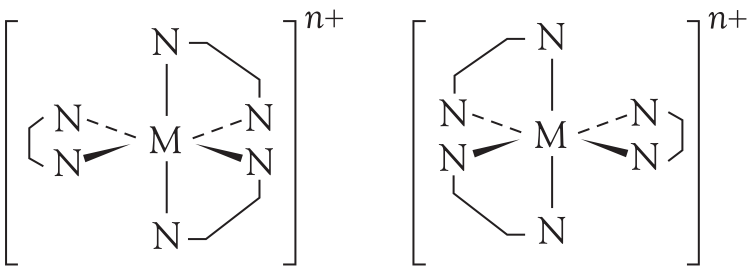
\includegraphics[width=0.9\textwidth]{figures/k19s507chiral.png}
\end{flashcard}



\begin{flashcard}[Teori]{Hvad er den primære begrænsning ved valens bindings teori?}
At teorien ikke kan forudsige men kun rationalisere
\end{flashcard}


\begin{flashcard}[Teori]{Hvilke antagelser gøres i krystalfeltteorien?}
Overgangsmetalionen er fri og på gasform.\\
Liganderne opfører sig som punktladninger.\\
Ingen interaktion mellem metallets $d$ orbitaler og ligandernes orbitaler.
\end{flashcard}


\begin{flashcard}[Teori]{Hvad er drivkraften for kompleksdannelse ifølge CFT?}
En fri gasformig metalions $d$ orbitaler har alle samme energiniveau (degenererede). Når liganderne binder aftager nogle af orbitalerne i energi mens andre vokser. Elektronerne fyldes i de nye lavere energiniveauer hvilket er energetisk favorabelt.
\end{flashcard}


\begin{flashcard}[Teori]{Hvad forstås ved CFSE?}
\textit{crystal felts stabilisations energi}. Den energi der udløses når elektroner går fra degerenrerede $d$ orbitaler til opsplittede $d$ orbitaler.
\end{flashcard}


\begin{flashcard}[Teori]{Hvad er sammenhængene mellem spin, felt og CFSE?}
Høj CFSE svarer til lavt spin hvilket svarer til et stærkt felt.
\end{flashcard}


\begin{flashcard}[Teori]{Hvilke faktorer har indflydelse på CFSE?}
Jo højere periode des højere CFSE.
Jo højere oxidationstrin des højere CFSE.
Jo flere ligander des højere CFSE.
Selve liganderne jvf. den spektrokemiske serie.
\end{flashcard}


\begin{flashcard}[Teori]{Opskriv den spektrokemiske serie}
\ce{I-} < \ce{Br-} < \ce{Cl-} < \ce{F-}\\< \ce{OH-} < \ce{OH2} < \ce{NH3} < \ce{en} < \ce{CN-} < \ce{CO}
\end{flashcard}


\begin{flashcard}[Teori]{Angiv hvorledes elektronerne fordeles i et oktaederiske kompleks}
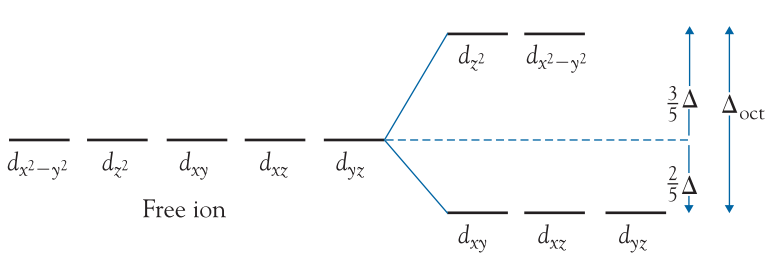
\includegraphics[width=0.9\textwidth]{figures/k19s513mooct.png}
\end{flashcard}


\begin{flashcard}[Teori]{Angiv hvorledes elektronerne fordeles i et tetraederisk kompleks}
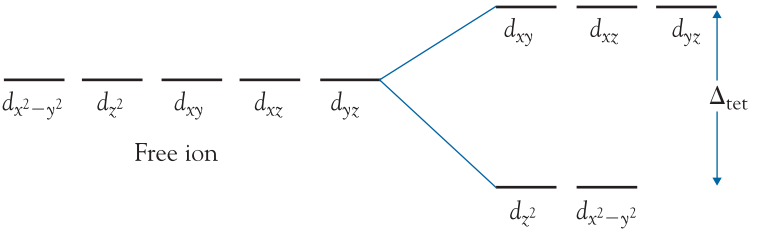
\includegraphics[width=0.9\textwidth]{figures/k19s516motet.png}
\end{flashcard}


\begin{flashcard}[Teori]{Angiv hvorledes elektronerne fordeles i et plankvadratisk kompleks}
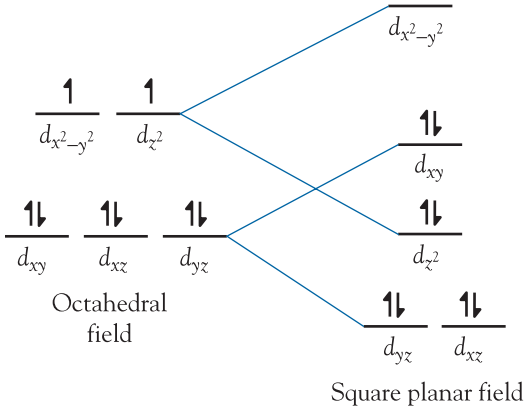
\includegraphics[width=0.8\textwidth]{figures/k19s517mopk.png}
\end{flashcard}


\begin{flashcard}[Teori]{Hvilken farve vil et kompleks have hvis det absorberer i den grønne del af det synlige spektrum?}
Det lys der ikke absorberes reflekteres. Derfor vil den reflektere en blanding af rød og blå dvs. lilla.
\end{flashcard}


\begin{flashcard}[Teori]{Hvilken farve vil du forvente et kompleks har hvis det har en høj CFSE?}
En farve der korresponderer til en kort bølgelængde hvilket svarer til energirig elektromagnetisk stråling. Eksempelvis faverne blå og violet.
\end{flashcard}


\begin{flashcard}[Egenskab]{Hvilke struktur har \ce{MgAl2O4}, \ce{Fe3O4}, \ce{Mn3O4} og \ce{MFe2O4} hvor M er dipositive overgangsmetalioner?}
Spinel, invers spinel, spinel og spinel.
\end{flashcard}


\begin{flashcard}[Teori]{Hvilke komplekser har oftest intense farver?}
Tetraederiske komplekser da de ikke har et symmetripunkt.
\end{flashcard}


\begin{flashcard}[Egenskab]{Forklar hvorfor permangernationen har en stærk farve}
Selvom ionen har en $d^{0}$ konfiguration kan der stadig ske elektronovergange via charge transfer fra oxygenatomets $p$ orbitaler til mangans ledige $d$ orbitaler.
\end{flashcard}


\begin{flashcard}[Teori]{Hvad forstås ved spinforbudte henholdsvis laporte forbudte elektronovergange?}
Spin: Sandsynligheden for ændring af spin er meget lille.\\
Laporte: Overgange mellem $d$ orbitaler er forbudte når molekylet har et inversionscenter.
\end{flashcard}


\begin{flashcard}[Egenskab]{Hvorfor er \ce{Cr^{3+}} og \ce{Co^{3+}} komplekser ofte inerte?}
De har 3 henholdsvis 6 $d$ elektroner i grundtilstanden. Med en oktaederisk konfiguration er de halvfyldte henholdsvis fyldte laveste $d$ energiniveauer så stabile at der ikke er aktiveringsenergien bliver høj.
\end{flashcard}


\begin{flashcard}[Teori]{Nævn tre typer af reaktioner til syntese af koordinationskomplekser og giv eksempler på dem}
Ligandudskiftning: \ce{[Ni(OH2)6]^{2+} + 6NH3 -> [Ni(NH3)6]^{2+} + 6H2O}\\\vspace*{0.5cm}
Redox:\\\ce{Os + 3F2 -> OsF6}\\\vspace*{0.5cm}
Partiel dekomponering: \ce{[Co(NH3)5(OH2)]Cl3 ->[\text{$\Delta$}] [Co(NH3)5Cl]Cl2 + H2O}
\end{flashcard}


\begin{flashcard}[Fremstilling]{Giv reaktionerne til fremstilling af bariumferrat(IV)}
\ce{2Fe^{3+} + 3ClO- + 10OH- -> 2FeO4^{2-} + 3Cl- + 5H2O}\\\vspace*{0.5cm}
\ce{FeO4^{2-} + Ba^{2+} -> BaFeO4(s)}
\end{flashcard}

\begin{flashcard}[Teori]{Hvad er grundprincippet i HSAB teori?
Angiv også 7 hårde, 2 mellem og 3 bløde ligandatomer}
Hårde ligander binder bedst til hårde overgangsmetaller.
Alle overgangsmetalioner med en ladning over +2 samt \ce{Mn^{+2}} er hårde, dem med +2 er mellem og alle med lavere ladning er bløde.\\\vspace*{0.3cm}
Hårde: \ce{C}, \ce{S}, \ce{As}, \ce{Se}, \ce{Te}, \ce{I}.\\
Mellem: \ce{Cl}, \ce{Br}.\\
Bløde: \ce{N}, \ce{O}, \ce{F}.  
\end{flashcard}


\begin{flashcard}[Teori]{Forklar begrebet \textit{kemisk symbiose}}
Et kompleks med bløde ligander har større tendens til at binde til en blød ligand mere end til at binde til en hård ligand og dermed opnå en "blanding".
Eksempelvis er \ce{[Co(NH3)5F]^{2+}} mere stabil end \ce{[Co(NH3)5I]^{2+}}
\end{flashcard}


\begin{flashcard}[Struktur]{Tegn strukturen af metalloporphyrinkomplekset}
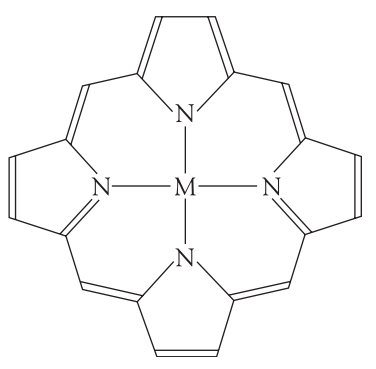
\includegraphics[width=0.6\textwidth]{figures/k19s529porphyrin.png}
\end{flashcard}
\cardfrontfoot{Kapitel 20}

\begin{flashcard}[Struktur]{Nævn alle plankvadratiske komplekser}
\ce{[PtCl4]^{2-}}, \ce{[Ni(CN)4]^{2-}}, \ce{[Pt(NH3)2Cl2]}, \ce{[Ni(DMG)2]}, \ce{[Cu(NH3)4]^{2+}} samt øvrige platin og palladium komplekser.\\\vspace*{0.5cm}
Alle andre komplekser med fire ligander er tetraederiske.
\end{flashcard}

\begin{flashcard}[Struktur]{Opskriv for hver af $3d$ overgangsmetallerne de oxidationstrin hvor det danner forbindelser med oxygen}
\begin{tabular}{l*{8}{c}r}
Ox.			& Ti & V & Cr & Mn & Fe & Co & Ni & Cu \\
\hline
1			&  &  &  &  &  &  &  & X \\
2			& X & X &  & X & X & X & X & X \\
2 \& 3		&  &  &  & X & X & X &  & \\
3			& X & X & X & X & X &  &  & \\
4			& X & X & X & X &  &  & X & \\
5			&  & X &  &  &  &  &  & \\
6			&  &  & X &  &  &  &  & \\
7			&  &  &  & X &  &  &  & \\
\end{tabular}
\end{flashcard}

\begin{flashcard}[Egenskab]{Hvilke tre overgangsmetaller danne alle stabile oxyanioner i sur opløsning?}
\ce{VO4^{3-}}, \ce{CrO4^{2-}} og \ce{MnO4^{-}} triaden
\end{flashcard}

\begin{flashcard}[Egenskab]{Hvilke tre overgangsmetaller danner alle tetrachloro komplekser?}
Fe, Co og Ni triaden
\end{flashcard}

\begin{flashcard}[Fremstilling]{Opskriv reaktionsligninger for hvordan rent titanium og titaniumdioxid fremstilles industrielt}
\ce{TiO2 + 2C + 2Cl2 ->[\text{$\Delta$}] TiCl4 + 2CO}\\\vspace*{0.5cm}
\ce{TiCl4 + 2Mg ->[\text{$\Delta$}] Ti + 2MgCl2}\\
eller\\
\ce{TiCl4 + O2 ->[\text{$\Delta$}] TiO2 + 2Cl2}
\end{flashcard}

\begin{flashcard}[Egenskab]{Angiv den primære mineralkilde til chrom}
Chromit, \ce{FeCr2O4}
\end{flashcard}

\begin{flashcard}[Egenskab]{Forklar hvorfor chromat- og dichromationen ikke er farveløse}
Charge transfer til oxygen.
\end{flashcard}

\begin{flashcard}[Reaktion]{Angiv ammoniumdichromats spontane reaktion ved antændelse}
\ce{(NH4)2Cr2O7 -> Cr2O3 + N2 + 4H2O(g)}
\end{flashcard}

\begin{flashcard}[Struktur]{Tegn strukturen af dichromationen}
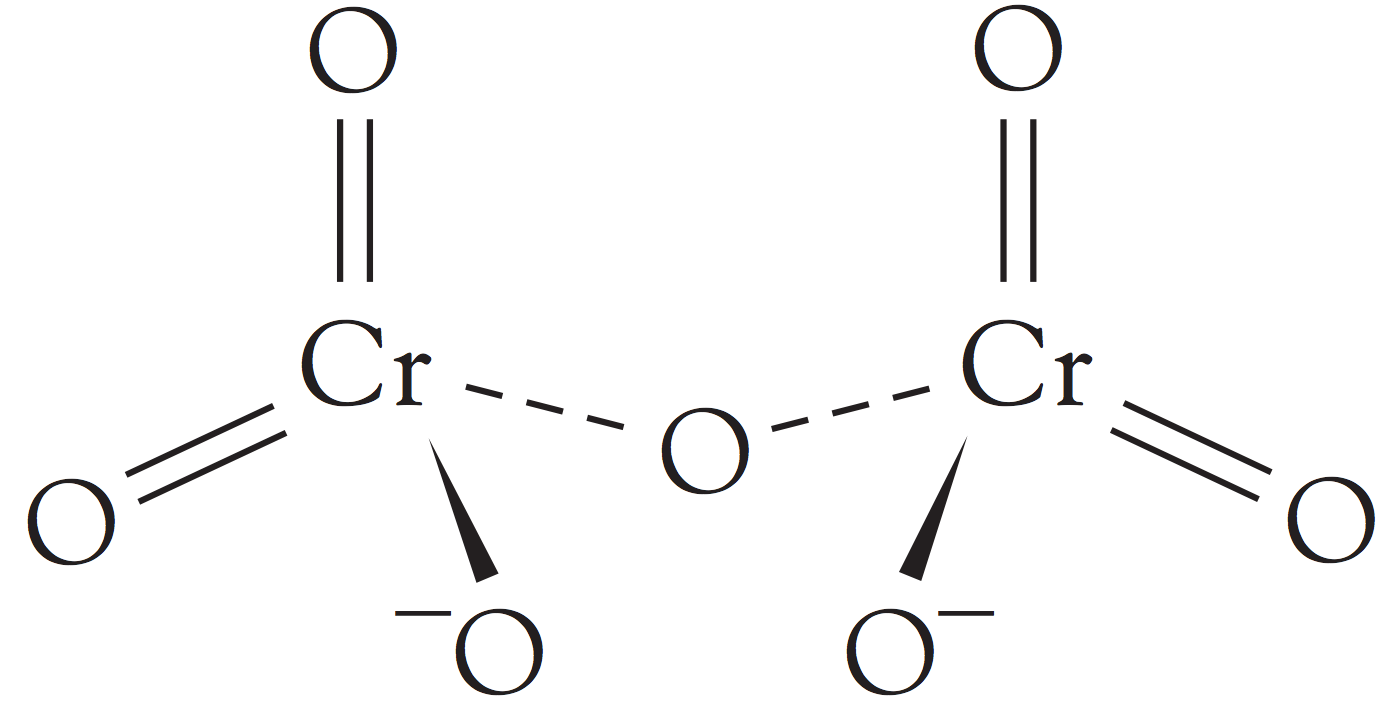
\includegraphics[width=0.9\textwidth]{figures/k20s540dichromat.png}
\end{flashcard}

\begin{flashcard}[Fremstilling]{Angiv hvordan dichromationen fremstilles industrielt}
\ce{4FeCr2O4 + 8Na2CO3 + 7O2 ->[\text{$\Delta$}] 8Na2CrO4 + 2Fe2O3 + 8CO2}\\\vspace*{0.5cm}
\ce{2Na2CrO4 + 2CO2 + H2O <=> Na2Cr2O7 + 2NaHCO3}
\end{flashcard}

\begin{flashcard}[Reaktion]{Angiv hvordan man kan undersøge om der er dichromat i en opløsning}
Dichromationen er orange men reagerer til en blå forbindelse ved tilsætning af hydrogenperoxid og ether.\\\vspace*{0.5cm}
\ce{Cr2O7^{2-} + 4H2O2 + 2H+ -> 2CrO(O2)2(ether) + 5H2O}
\end{flashcard}

\begin{flashcard}[Struktur]{Tegn strukturen af chromylchlorid}
\schemestart
$\chemfig{Cr(=[2]\ce{O})(=[5]\ce{O})(<[:-50]\ce{Cl})(<:[:-12]\ce{Cl})}$
\schemestop
\end{flashcard}

\begin{flashcard}[Fremstilling]{Angiv med en reaktionsligning hvordan man kan fremstille chromylchlorid}
\ce{K2Cr2O7 + 4NaCl + 6H2SO4 -> 2CrO2Cl2 + 2KHSO4 + 4NaHSO4 + 3H2O}
\end{flashcard}

\begin{flashcard}[Reaktion]{Angiv chromylchlorids reaktion i basisk væske}
\ce{CrO2Cl2 + 4OH- -> CrO4^{2-} + 2Cl- + 2H2O}
\end{flashcard}

\begin{flashcard}[Fremstilling]{Hvordan kan man fremstille chrom(VI)oxid?}
\ce{K2Cr2O7 + H2SO4 + H2O -> K2SO4 + "H2CrO4"}\\\vspace*{0.5cm}
\ce{"H2CrO4" -> CrO3 + H2O}
\end{flashcard}

\begin{flashcard}[Anvendelse]{Angiv en karakteristisk anvendelse af chrom(III)oxid}
Chrom(III)oxid er et grønt fast stof som ikke er opløseligt i vand. Derfor anvendes det som pigment i amerikanske dollars.
\end{flashcard}

\begin{flashcard}[Egenskab]{Hvad er den primære mineralkilde til mangan?}
\ce{Mn7SiO12}
\end{flashcard}

\begin{flashcard}[Reaktion]{Kaliumpermangernat kan oxidere saltsyre. Angiv reaktionsligningen}
\ce{2KMnO4 + 16HCl -> 2KCl + 2MnCl2 + 8H2O + 5Cl2}
\end{flashcard}

\begin{flashcard}[Egenskab]{Hvorfor er \ce{Mn^{2+}} næsten farveløs?}
I high spin konfigurationen kan der kun ske elektronovergange ved at vende spinnet af en elektron og parre den med en anden. Sandsynligheden for dette er ekstremt lav da det er en spin forbudt elektronovergang.
\end{flashcard}

\begin{flashcard}[Reaktion]{Mangan(II)hydroxid kan reagere med oxygen. Giv reaktionsligningen}
\ce{4Mn(OH)2(s) + O2 -> 4MnO(OH)(s) + 2H2O}
\end{flashcard}

\begin{flashcard}[Reaktion]{Vis med reaktionsligninger hvorledes man kan undersøge om en opløsning indeholder \ce{Mn^{2+}}}
\ce{2Mn^{2+} + 5 [BiO3]- + 14H+ -> 2MnO4- + 5Bi^{3+} + 7H2O}
\end{flashcard}

\begin{flashcard}[Reaktion]{\ce{Mn2O7} dekomponerer eksplosivt. Giv reaktionsligningen}
\ce{2Mn2O7(l) -> 4MnO2 + 3O2}
\end{flashcard}

\begin{flashcard}[Reaktion]{Ionisk mangan(IV)oxid kan bruges til at fremstille chlorgas. Giv reaktionsligningen}
\ce{MnO2 + 4HCl -> MnCl2 + Cl2 + 2H2O}
\end{flashcard}

\begin{flashcard}[Anvendelse]{Mangan kan anvendes i alkaliske batterier. Opskriv halvcellereaktionerne}
\ce{2MnO2 + 2H2O + 2e- -> 2MnO(OH) + 2OH-}\\
\ce{Zn + 2OH- -> Zn(OH)2(s) + 2e-}
\end{flashcard}

\begin{flashcard}[Fremstilling]{Opskriv reaktionsligningerne til industriel fremstilling af jern ud fra jernmalm i en højovn}
\ce{2C + O2 -> 2CO}\\
\ce{3Fe2O3 + CO -> 2Fe3O4 + CO2}\\
\ce{Fe3O4 + CO -> 3FeO + CO2}\\
\ce{CaCO3 ->[\text{$\Delta$}] CaO + CO2}\\
\ce{FeO + CO -> Fe + CO2}\\
Slagger dannes
\ce{CaO + SiO2 -> CaSiO3}\\
\end{flashcard}

\begin{flashcard}[Fremstilling]{Opskriv reaktionsligningerne til industriel fremstilling af jern ud fra jernmalm af høj kvalitet ved DRI metoden}
\ce{Fe3O4 + CO -> 3FeO + CO2}\\
\ce{Fe3O4 + H2 -> 3FeO + H2O}\\
\ce{FeO + CO -> Fe + CO2}\\
\ce{FeO + H2 -> Fe + H2O}\\
Hydrogen til processen fremstilles via methan reforming\\
\ce{CH4 + CO2 -> 2CO + 2H2}\\
\ce{CH4 + H2O -> CO + 3H2}\\
\end{flashcard}

\begin{flashcard}[Struktur]{Tegn strukturen af \ce{Fe2Cl6}}
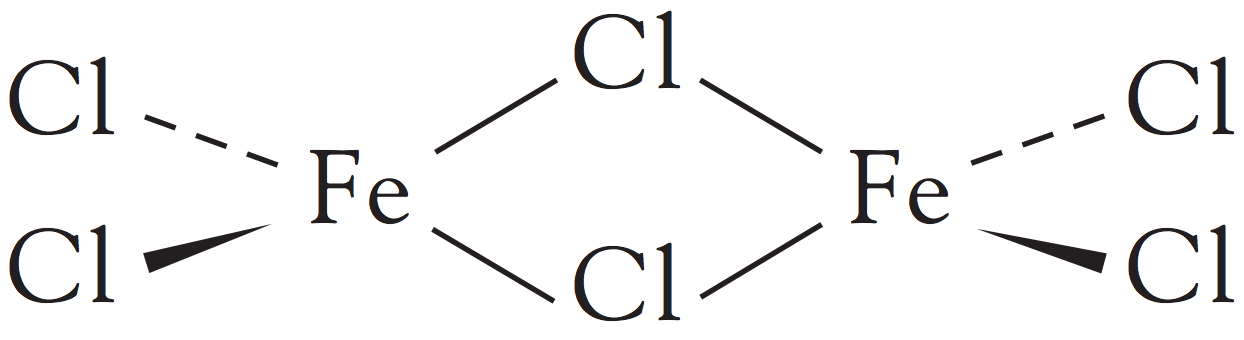
\includegraphics[width=0.9\textwidth]{figures/k20s553fe2cl6.png}
\end{flashcard}

\begin{flashcard}[Reaktion]{Jern kan reagere med chlorgas. Giv reaktionen samt produktets reaktion med vand}
\ce{2Fe + 3Cl2 -> 2FeCl3}\\\vspace*{0.5cm}
\ce{FeCl3 + 3H2O -> Fe(OH)3 + 3HCl(g)}
\end{flashcard}

\begin{flashcard}[Egenskab]{Jern(III) salte regarer ofte surt når de opløses i vand. Hvorfor?}
Ligesom aluminium kan jern koordinere vandmolekyler. På grund af den høje ladningstæthed kan vandmolekylerne binde så stærkt at de kan reagere surt.\\
Eksempelvis:\\
\ce{[Fe(OH2)6]^{3+} + H2O <=> H3O+ + [Fe(OH2)5OH]^{2+}}
\end{flashcard}

\begin{flashcard}[Reaktion]{Jern(III) og jern(II) giver bundfald i basisk væske. Opskriv reaktionsligningerne}
\ce{Fe^{3+} + 3OH- -> FeO(OH) + H2O}\\
Produktet af ovenstående kaldes i daglig tale rust
\ce{Fe^{2+} + 2OH- -> Fe(OH)2}
\end{flashcard}

\begin{flashcard}[Fremstilling]{Angiv reaktionsligningen for industriel fremstilling af jern(II)chlorid}
\ce{Fe + 2HCl(g) -> FeCl2 + H2}
\end{flashcard}

\begin{flashcard}[Reaktion]{Jern(II) og jern(III) kan påvises ved to forskellige lignende metoder der begge giver berlinerblåt. Opskriv reaktionsligningerne}
\ce{3Fe^{2+} + 4[Fe(CN)6]^{3-} -> Fe4[Fe(CN)6]3 + 6CN-}\\\vspace*{0.5cm}
\ce{4Fe^{3+} + 3[Fe(CN)6]^{4-} -> Fe4[Fe(CN)6]3}
\end{flashcard}

\begin{flashcard}[Reaktion]{Opskriv reaktionsligningerne for dannelse af rust}
\ce{2Fe + O2 + 2H2O -> 2Fe(OH)2}\\\vspace*{0.5cm}
\ce{4Fe(OH)2 + O2 -> 4FeO(OH) + 2H2O}
\end{flashcard}

\begin{flashcard}[Reaktion]{Kobolt(II) kan bundfældes med en svag opløsning af stærk base. Herefter går det i opløsning ved kontakt med luft. Giv reaktionsligningerne}
\ce{Co^{2+} + 2OH- -> Co(OH)2}\\\vspace*{0.5cm}
\ce{4Co(OH)2 + O2 -> 4CoO(OH) + 2H2O}
\end{flashcard}

\begin{flashcard}[Fremstilling]{Opskriv reaktionen for oprensning af nikkel ved Mond processen}
\ce{Ni + 4CO <=> Ni(CO)4}\\\vspace*{0.5cm}
Reaktionen er forskudt mod højre ved forholdsvis lave temperaturer
\end{flashcard}

\begin{flashcard}[Egenskab]{Nikkel(II) kan bundfældes med base. Opskriv reaktionen}
\ce{Ni^{2+} + 2OH- -> Ni(OH)2(s)}
\end{flashcard}

\begin{flashcard}[Fremstilling]{Angiv den primære kilde til kobber og hvordan kobberet kan udvindes ved en pyrometallurgisk proces}
\ce{4CuFeS2 + 9O2 -> 2Cu2S + 6SO2 + 2Fe2O3}\\
\ce{Fe2O3 + 3SiO2 -> Fe2(SiO2)3}\\
\ce{2Cu2S + 3O2 -> 2Cu2O + 2SO2}\\
\ce{Cu2S + 2Cu2O -> 6Cu + SO2}
\end{flashcard}

\begin{flashcard}[Fremstilling]{Opskriv reaktionsligningen for udvinding af kobber fra \ce{CuFeS2} ved en hydrometallurgisk proces}
\ce{2CuFeS2 + H2SO4 + 4O2 -> 2CuSO4(aq) + 3S + Fe2O3 + H2O}\\
Kobberet oprenses ved elektrolyse
\end{flashcard}

\begin{flashcard}[Egenskab]{Forklar med udgangspunkt i kobber(II) hvad der forstås ved Jahn-Teller effekten}
$d_{x^2-y^2}$ og $d_{z^2}$ opsplittes i energi fordi der er et ulige antal $d$ elektroner (9) hvorved de to bindinger langs $z$-aksen forlænges.
\end{flashcard}

\begin{flashcard}[Fremstilling]{Hvorledes kan man fremstille kobber(I)chlorid?}
\ce{2Cu + 2H+ -> 2Cu+ + H2}\\
\ce{Cu+ + 2Cl- <=> [CuCl2]-}\\
\ce{[CuCl2]- -> CuCl + Cl-}
\end{flashcard}
\cardfrontfoot{Kapitel 21}

\begin{flashcard}[Teori]{Forventes 4-6 periode overgangsmetallerne at være lav spin eller høj spin?}
Lav spin da CFSE vokser ned gennem perioderne.
\end{flashcard}

\begin{flashcard}[Teori]{Hvad forstås ved \textit{lanthanoid contraction}?}
Elektronerne i $f$ orbitaler skærmer i meget ringe grad for de ydre elektroner som så oplever en stærkere tiltrækning fra kernen hvilket fører til en lavere ionradius. Derfor har overgangsmetallerne i 6. periode næsten samme radius og dermed ladningstæthed som dem i 5. periode.
\end{flashcard}

\begin{flashcard}[Fremstilling]{Hvordan fremstilles sølv industrielt?}
\ce{2AgS + 8CN- + O2 + 2H2O -> 4[Ag(CN)2]- + 2S + 4OH-}\\\vspace*{0.5cm}
\ce{2[Ag(CN)2]- + Zn -> 2Ag + [Zn(CN)4]^{2-}}
\end{flashcard}

\begin{flashcard}[Reaktion]{Der tilføjes sølvioner til en opløsning der enten indeholder iodid, bromid eller chlorid ioner. Hvordan kan man de eneklte ioner?}
Sølvchlorid er opløseligt i fortyndet ammoniak mens sølvbromid er opløseligt i koncentreret ammoniak. Sølviodid er ikke opløseligt i ammoniak.\\\vspace*{0.5cm}
\ce{AgCl + 2NH3 -> [Ag(NH)2]+ + Cl-}\\
\ce{AgBr + 2NH3[konc] -> [Ag(NH)2]+ + Br-}
\end{flashcard}
\cardfrontfoot{Kapitel 22}

\begin{flashcard}[Struktur]{Giv reaktionsligningen for forbrænding af zink i chlorgas}
\ce{Zn + Cl2(g) -> ZnCl2(g)}
\end{flashcard}

\begin{flashcard}[Fremstilling]{Giv reaktionsligningerne for industriel fremstilling af zink}
\ce{2ZnS + 3O2 ->[\text{$\Delta$}] 2ZnO + 2SO2}\\\vspace*{0.5cm}
\ce{ZnO + C ->[\text{$\Delta$}] Zn + CO}
\end{flashcard}

\begin{flashcard}[Egenskab]{Forklar hvorfor zink kan beskytte fjern mod korrosion}
Reduktionspotentialet for zink er lavere end det er for jern. Derfor korroderer zink først hvilket efterlader jern intakt.
\end{flashcard}

\begin{flashcard}[Egenskab]{Hvordan kan \ce{Zn(OH)2} bringes i opløsning?}
Ved tilsætning af base i form af hydroxidioner eller ammoniak.\\\vspace*{0.5cm}
\ce{Zn(OH)2 + 2OH- -> [Zn(OH)4]^{2-}}\\
\ce{Zn(OH)2 + 4NH3 -> [Zn(NH3)4]^{2+} + 2OH-}
\end{flashcard}

\begin{flashcard}[Fremstilling]{Opskriv to metoder til fremstilling af zinkoxid}
\ce{2Zn + O2 -> 2ZnO}\\\vspace*{0.5cm}
\ce{ZnCO3 ->[\text{$\Delta$}] ZnO + CO2}
\end{flashcard}

\begin{flashcard}[Anvendelse]{Opskriv halvcellereaktionerne i et NiCad batteri}
\ce{Cd + 2OH- -> Cd(OH)2 + 2e-}\\\vspace*{0.5cm}
\ce{2NiO(OH) + 2H2O + 2e- -> 2Ni(OH)2 + 2OH-}
\end{flashcard}

\begin{flashcard}[Fremstilling]{Angiv med reaktionsligning hvordan kviksølv fremstilles industrielt}
\ce{HgS + O2 ->[\text{$\Delta$}] Hg + SO2}
\end{flashcard}

\begin{flashcard}[Fremstilling]{Hvordan kan man fremstille kviksølv(II)chlorid og kviksølv(I)chlorid?}
\ce{Hg + Cl2(g) -> HgCl2}\\\vspace*{0.5cm}
\ce{2HgCl2 + SnCl2 -> SnCl4 + Hg2Cl2}\\
Tilsættes overskud af tin(II)chlorid fås kviksølv\\
\ce{Hg2Cl2 + SnCl2 -> SmCl4 + 2Hg}
\end{flashcard}

\begin{flashcard}[Reaktion]{Hvilken reaktion finder sted når kviksølvoxid opvarmes kraftigt?}
\ce{2HgO ->[\text{$\Delta$}] 2Hg + O2}
\end{flashcard}

\begin{flashcard}[Anvendelse]{Giv halvcellereaktionerne der finder sted i et kviksølv batteri}
\ce{Zn + 2OH- -> Zn(OH)2 + 2e-}\\\vspace*{0.5cm}
\ce{HgO + H2O + 2e- -> Hg + 2OH-}
\end{flashcard}

\begin{flashcard}[Egenskab]{Kobber(I), guld(I) og \ce{Hg2^{2+}} ionen har tendens til at disproportionere. Giv reaktionsligningerne}
\ce{2Cu+ -> Cu2+ + Cu}\\\vspace*{0.5cm}
\ce{3Au+ -> 2Au + Au^{3+}}\\\vspace*{0.5cm}
\ce{Hg2^{2+} <=> Hg + Hg^{2+}}\\
Da ovenstående er en ligevægt kan den forskydes mod højre ved at fælde kviksølv(II) ionerne med sulfid.
\end{flashcard}

\begin{flashcard}[Egenskab]{Opskriv de tungtopløselige hydroxider af $d$ metallerne samt hvorvidt de er amfotere eller ej}
Ikke amfotere: \ce{Mn(OH)2}, \ce{MnO(OH)}, \ce{Fe(OH)2}, \ce{FeO(OH)}, \ce{Ni(OH)2}, \ce{NiO(OH)}, \ce{Cd(OH)2}\\\vspace*{0.5cm}
Amfotere: \ce{Co(OH)2}, \ce{Cu(OH)2}, \ce{Zn(OH)2}\\
Der dannes tetraedriske komplekser når ovenstående reagerer med stærk base.
\end{flashcard}
\cardfrontfoot{Kapitel 23}

\begin{flashcard}[Teori]{Hvad forstås ved en organometallisk forbindelse?}
En forbindelse hvor der er mindst en covalent binding mellem et metal atom og et carbon atom.
\end{flashcard}

\begin{flashcard}[Teori]{Hvad betyder det hvis en metal-carbon binding er di-, tetra- eller hexahapto?}
At metallet binder til to, fire eller seks carbonatomer på én gang.
\end{flashcard}

\begin{flashcard}[Teori]{Hvad er forskellen mellem $\mu$ og $\eta$ mht. hapticitet?}
$\mu$ angiver antallet af carbonatomer der binder covalent til et metalatom. $\eta$ angiver Antallet af metal atomer et carbon atom binder til.
\end{flashcard}

\begin{flashcard}[Teori]{Opskriv de fire forskellige typer elementarreaktioner}
\begin{enumerate}
\item Oxidativ addition\\M går typisk 2 op i oxidationstrin, antal ligander vokser med 2
\item Reduktiv elimination\\ M går typisk 2 ned i oxidationstrin, antal ligander aftager med 2
\item Insertion
\item Ligand substitution
\end{enumerate}
\end{flashcard}
\end{document}